\documentclass[10pt, a4paper, oneside, fontset=none]{ctexart}
%调用宏包
\usepackage{amsmath, amsthm, amssymb, graphicx, wrapfig, mathrsfs, upgreek}
\usepackage[bookmarks=true, colorlinks, citecolor=blue, linkcolor=black]{hyperref}
\usepackage{color, framed, geometry, tcolorbox, multirow, booktabs}
\tcbuselibrary{breakable}%box跨页
\tcbuselibrary{skins}%box跨页不留边
%\usepackage{CJKpunct}
\usepackage{marginnote}
\usepackage{makecell, booktabs, longtable}
\usepackage[font=sf, labelfont+=bf]{caption}
\usepackage[font={small, sf}]{subfig}
\usepackage{multicol}
\usepackage{arydshln, nicematrix}%矩阵
\usepackage{extarrows}
\usepackage[american, cuteinductors, ]{circuitikz}
\usepackage{xpatch}
\usepackage{rotating}%旋转
\usepackage{physics}
\usepackage{siunitx}
\usepackage{enumitem}
\usepackage{listings}
\usepackage[text=\includegraphics{C:/Users/16870/.vscode/LaTeX_Application/tex/23Au/图标简稿.png},angle=0]{draftwatermark}%水印
%\usepackage{tikz}
%基本字体设置
\usepackage[math-style=ISO, bold-style=ISO]{unicode-math}
%\setmainfont{EB Garamond}
%\setmathfont{Garamond-Math.otf}[StylisticSet={7,9}]
\setmonofont{Iosevka}
\setmathfont{latinmodern-math.otf}
%\setmathfont[range=bb]{TeXGyrePagellaMath-Regular}
%\setmathsfont(Digits,Latin){Garamond MT Pro}
\setCJKmainfont{方正书宋_GBK}[BoldFont={思源宋体 CN Bold}, ItalicFont=方正楷体_GBK, BoldItalicFont={汉仪颜楷W}]
\setCJKsansfont{汉仪文黑-45W ExtraLight}[BoldFont={汉仪文黑-75W Bold}, ItalicFont={方正颜真卿楷书 简繁}]
\setCJKmonofont{LXGWNeoXiHei.ttf}
%附加字体设置
\newCJKfontfamily{\kaico}{可口可乐在乎体 楷体}
\newCJKfontfamily{\kai}{方正楷体_GBK}[BoldFont={汉仪颜楷W}, ItalicFont={方正清刻本悦宋 简繁}, BoldItalicFont={方正颜真卿楷书 简繁}]
\newCJKfontfamily{\yan}{方正清刻本悦宋 简繁}[ItalicFont={方正颜真卿楷书 简繁}]
\newCJKfontfamily{\xiu}{方正宋刻本秀楷_GBK}[ItalicFont={方正宋刻本秀楷_GBK}, BoldFont={方正颜真卿楷书 简繁}]
\newCJKfontfamily{\run}{汉仪润圆-45W}[BoldFont=汉仪润圆-75W, ItalicFont={汉仪润圆-45W}]
\newCJKfontfamily{\wen}{汉仪文黑-45W ExtraLight}[BoldFont={汉仪文黑-75W Bold}, ItalicFont={汉仪文黑-85W Heavy}]
%文档格式
\geometry{left=2.24cm, right=2.24cm, top=3.18cm, bottom=3.18cm}
\linespread{1.4}
\numberwithin{equation}{section}
\setcounter{tocdepth}{3}
\setcounter{secnumdepth}{4}
\renewcommand{\theparagraph}{\Alph{paragraph})}
\newcommand{\Section}[1]{ \refstepcounter{section} \section*{*\thesection\texorpdfstring{\quad}{} #1} \addcontentsline{toc}{section}{\makebox[0pt][r]{*}\thesection\texorpdfstring{\quad}{} #1} }
\newcommand{\Subsection}[1]{ \refstepcounter{subsection} \subsection*{*\thesubsection\texorpdfstring{\quad}{} #1} \addcontentsline{toc}{subsection}{\makebox[0pt][r]{*}\thesubsection\texorpdfstring{\quad}{} #1} }
\newcommand{\Subsubsection}[1]{ \refstepcounter{subsubsection} \subsubsection*{*\thesubsubsection\texorpdfstring{\quad}{} #1} \addcontentsline{toc}{subsubsection}{\makebox[0pt][r]{*}\thesubsubsection\texorpdfstring{\quad}{} #1} }
\setlist[itemize]{leftmargin=3em, labelsep=0.25em, itemindent=0em, itemsep=0pt, parsep=0pt, topsep=3pt, partopsep=0pt}
\setlength{\marginparwidth}{8em}
\setlength{\lineskip}{5pt}
\setlength{\lineskiplimit}{5pt}

\setlength{\abovecaptionskip}{0.3em}
\setlength{\belowcaptionskip}{0em}
\captionsetup[subfigure]{captionskip=0.5em, nearskip=0em}
\captionsetup[table]{justification=raggedright,singlelinecheck=false}
\renewcommand{\thefigure}{\thesection.\arabic{figure}}
\renewcommand{\thetable}{\thesection.\arabic{table}}

\tikzset{every node/.style={scale=0.8}}
\ctikzset{monopoles/vcc/arrow={Stealth[width=4pt, length=6pt]}}
\ctikzset{monopoles/vee/arrow={Stealth[width=4pt, length=6pt]}}
\ctikzset{bipoles/length=1cm} %电路图大小标的
\ctikzset{resistors/thickness=2.5}
\ctikzset{voltage=raised}
\ctikzset{bipoles/cuteswitch/thickness=0.4}
\tikzset{
    R/.append style={color=balib},
    C/.append style={color=balib},
    L/.append style={color=balib},
    battery1/.append style={color=meihongb},
    battery2/.append style={color=meihongb},
    battery/.append style={color=meihongb},
}
\tikzset{bcirc/.style={circ, color=black}}
\ctikzset{*-*/.style = {bipole nodes={bcirc}{bcirc}}}
\ctikzset{-*/.style = {bipole nodes={none}{bcirc}}}
\ctikzset{*-/.style = {bipole nodes={bcirc}{none}}}
%\punctstyle{kaiming}
%定理环境
\theoremstyle{plain}
\newtheorem{theorem}{定理}[subsection]
\newtheorem{definition}{定义}[subsection]
\newtheorem{lemma}[theorem]{引理}
\newtheorem{corollary}[theorem]{推论}
\newtheorem{proposition}[theorem]{命题}

\theoremstyle{definition}
\newtheorem{example}[theorem]{例}
\newtheorem{circum}[theorem]{情形}

\newenvironment{proofs}[1][\small\proofname]{\begin{pf}[breakable, enhanced jigsaw]\begin{proof}[#1]\small\kai
	\abovedisplayskip=2pt
	\belowdisplayskip=2pt
}{\end{proof}\end{pf}}
\newenvironment{solution}[1][解]{\begin{proofs}[\small\textit{\yan #1}]\renewcommand{\qedsymbol}{$\circledS$}}{\end{proofs}}
\renewcommand{\proofname}{\yan{证明}}

\renewenvironment{cases}[1][l]{\left\{\,\begin{NiceArray}{#1}}{\end{NiceArray}\right.}
%颜色命名
\definecolor{meihong}{rgb}{0.85,0.2,0.47}
\definecolor{bali}{rgb}{0.2,0.6,0.78}
\definecolor{qinglv}{rgb}{0,0.35,0.32}
\definecolor{meihongb}{rgb}{0.85,0.2,0.47}
\definecolor{balib}{rgb}{0.15,0.45,0.58}
\definecolor{qinglvb}{rgb}{0,0.35,0.32}
%box环境
\newtcolorbox{pr}[2][]
{colback=black!5!white,colframe=white!75!black,fonttitle=\sffamily\wen\bfseries,title=#2,#1}
\newtcolorbox[use counter=definition,number within=subsection]{defi}[2][]
{colback=bali!5!white,colframe=bali!75!black,fonttitle=\sffamily\wen\bfseries,title=定义~\thetcbcounter. #2,#1}
\newtcolorbox[auto counter,number within=section]{compl}[2][]
{colback=bali!5!white,colframe=bali!65!black,fonttitle=\sffamily\wen\bfseries,label=#2,title=元件~\thetcbcounter. #2,#1, fontupper=\kai, fontlower=\kai}
\newtcolorbox[use counter=theorem,number within=subsection]{theo}[2][]
{%grow to right by=3.2cm,
colback=meihong!5!white,colframe=meihong!75!black,fonttitle=\sffamily\wen\bfseries,fontupper=\run,title=结论~\thetcbcounter. #2,#1}
\newtcolorbox[use counter=definition,number within=subsection]{defil}[2][]
{colback=bali!5!white,colframe=bali!75!black,fonttitle=\sffamily\wen\bfseries,label=#2,title=定义~\thetcbcounter. #2,#1}
\newtcolorbox[use counter=theorem,number within=subsection]{theol}[2][]
{%grow to right by=3.2cm,
colback=meihong!5!white,colframe=meihong!75!black,fonttitle=\sffamily\wen\bfseries,fontupper=\run,label=#2,title=结论~\thetcbcounter. #2,#1}
\newtcolorbox[auto counter,number within=section]{note}[2][]
{colback=qinglv!5!white,colframe=qinglv!75!black,fonttitle=\sffamily\wen\bfseries,title=注~\thetcbcounter. #2,#1}
\newtcbox{\prenote}[1][]
{left=0.25em,right=0.25em,top=0.25em,bottom=0.25em,width=8.5em,toptitle=0.1em,before skip=0pt,after skip=3pt,colback=gray!5!white,colframe=gray!50!black,fonttitle=\linespread{1}\raggedright\small\sf\bfseries,fontupper=\linespread{1}\small\sf,title=#1}
\newtcolorbox{pf}[1][]
{colback=black!5!white,colframe=white!75!black,#1}
\newtcolorbox{eq}[1][]
{standard jigsaw, colback=meihong!5!white, opacityback=0.7, %grow to right by=3.2cm, 
colframe=meihong!85!black,#1, boxrule=0.4pt, leftrule=10pt, arc=0pt, before skip=7pt, after skip=7pt}
%\newcommand{\mybox}[1]{\tikz[baseline=(MeNode.base)]{\node[rounded corners, fill=gray!20](MeNode){#1};}}

\lstset{
	xleftmargin=3em, xrightmargin=1em, 
	breaklines,                                 % 自动将长的代码行换行排版
	extendedchars=false,                        % 解决代码跨页时,章节标题,页眉等汉字不显示的问题
	rulecolor=\color[rgb]{0.8,0.8,0.8},         % 设置代码框颜色
	backgroundcolor=\color[rgb]{0.96,0.96,0.96},% 背景颜色
	keywordstyle=\colors{bali}\bfseries,        % 关键字颜色
	identifierstyle=\color{black},              % 普通标识符颜色
	commentstyle=\rm\kai\color{gray},          	% 注释颜色
	stringstyle=\colors{meihong},      			% 字符串颜色
	showstringspaces=false,                     % 不显示字符串内的空格
	numbers=left,                               % 显示行号
	numberstyle=\tiny,              			% 设置数字字体
	basicstyle=\linespread{1}\tt,               % 设置基本字体
	captionpos=t,                               % title在上方(在bottom即为b)
	frame=single,                               % 设置代码框形式
	showtabs=false, 
	numbersep=15pt, 
	framesep=1em, 
	language=C++, 
	columns=flexible, 
	tabsize=4, 
}

\catcode`\,=\active
\def ,{\textup{,}\hskip0.5em }
\newcommand{\hang}[1][1]{\hangafter 1 \hangindent #1em \noindent}
\newcommand{\page}[1]{\hfill P$_\text{#1}$}
\newcommand{\colors}[1]{\color{#1!75!black}}
\newcommand{\paratitle}[1]{\hang \textbf{\wen #1}\hskip1em}
\newcommand{\tboqi}[1]{\textbf{\xiu\color{qinglv!75!black}#1}}
\newcommand{\mboqi}[1]{\symbf{\xiu\color{qinglv!75!black}#1}}
\newcommand{\tboba}[1]{\textbf{\kai\color{bali!75!black}#1}}
\newcommand{\mboba}[1]{\symbf{\kai\color{bali!75!black}#1}}
\newcommand{\tbome}[1]{\textbf{\run\run\color{meihong!75!black}#1}}
\newcommand{\mbome}[1]{\run\symbf{\run\color{meihong!75!black}#1}}
\newcommand{\adjline}{	\lineskiplimit=3pt
	\lineskip=3pt
	\abovedisplayskip=6pt
	\belowdisplayskip=6pt 
	}
\newcommand{\den}[2][]{\begin{defi}{#1}\adjline
	\kai #2\end{defi}}
\newcommand{\din}[2][]{\begin{theo}{#1}\adjline
	\run #2\end{theo}}
\newcommand{\de}[2][]{\begin{defil}{#1}\adjline
	\kai #2\end{defil}}
\newcommand{\di}[2][]{\begin{theol}{#1}\adjline
	\run #2\end{theol}}
\newcommand{\dep}[3][]{\begin{defi}{#1\page{#2}}\adjline
	\kai #3\end{defi}}
\newcommand{\dip}[3][]{\begin{theo}{#1\page{#2}}\adjline
	\run #3\end{theo}}
\newcommand{\zhu}[2][]{\begin{note}{#1}\adjline
	\xiu #2\end{note}}
\newcommand{\bu}[3][]{\begin{compl}{#1}	\paratitle{记号}#2 \tcblower\paratitle{特性}#3\end{compl}}
\newcommand{\trans}[2][注]{\begin{wrapfigure}{r}{8.7em}
		\vspace{-1.5em}
		\prenote[#1]{\makebox[8em][l]{#2}}
	\end{wrapfigure}}
% \newcommand{\tranS}[3][-1]{\marginnote{
% 		\begin{prenote}{#2}
% 			\raggedright
% 			#3
% 		\end{prenote}
% 	}[#1\baselineskip]}
\newcommand{\cbox}[2][]{
	$\vcenter{\hbox{\begin{circuitikz}[#1]
		#2
	\end{circuitikz}}}$
	}
\newcommand{\shbox}[1]{\cbox{\draw (0,0) to[#1] (1.5,0);}(\texttt{#1})}
%定义算符
\newcommand{\rref}{\symup{rref}}
\newcommand{\C}{\mathbb{C}}
\renewcommand{\i}{\symsf{j}}
\newcommand{\neiji}[4]{\symbf{#1}_{#3}^\symup{T}\symbf{#2}_{#4}}
\def\upint{\mathchoice%
	{\mkern13mu\overline{\vphantom{\intop}\mkern7mu}\mkern-20mu}%
	{\mkern7mu\overline{\vphantom{\intop}\mkern7mu}\mkern-14mu}%
	{\mkern7mu\overline{\vphantom{\intop}\mkern7mu}\mkern-14mu}%
	{\mkern7mu\overline{\vphantom{\intop}\mkern7mu}\mkern-14mu}%
	\int}
\def\lowint{\mkern3mu\underline{\vphantom{\intop}\mkern7mu}\mkern-10mu\int}
\renewcommand{\a}[1]{\left\langle #1 \right\rangle}
\renewcommand{\v}{\vee}
\newcommand{\A}{\wedge}
\renewcommand{\c}[1]{\symbfsfit{#1}}
\newcommand{\V}{\c{V}}
\newcommand{\I}{\c{I}}
\newcommand{\G}{\c{G}}
\newcommand{\Lr}{\Leftrightarrow}
\newcommand{\LLr}[2][]{\xLongleftrightarrow[#1]{#2}}
\newcommand{\rl}{\rightleftarrows}
\newcommand{\dif}{\mathop{}\!\symup{d}}
\newcommand{\Dif}{\mathop{}\!\symup{\Delta}}
\newcommand{\e}{\symup{e}}
\newcommand{\R}{\mathbb{R}}
\newcommand{\bF}{\mathbb{F}}
\newcommand{\dint}{\displaystyle\int}
\newcommand{\dt}[1][]{\dfrac{\dif #1}{\dif t}}
\renewcommand{\ang}[1]{\vcenter{\hbox{\begin{tikzpicture}
	\node (box) at (0,0) {$#1$};
	\draw (box.south west) ++ (-0.05,0.08) coordinate(left)
	(box.south east) ++ (-0.1,0.08) -- (left) -- ++ (0.17,0.45);
\end{tikzpicture}}}\!\!}
\newcommand{\meshcurrent}[2]{\draw[latex-] #1 node{#2} +(0.43,0.25) arc(30:330:0.5);
}
\newcommand{\equ}[1]{\begin{eq}
%	\setmathfont{GFSNeohellenicMath.otf}
	\setmathfont{FiraMath-Regular.otf}\sffamily
	\begin{equation}
		{\color{meihong!85!black} #1}
	\end{equation}\end{eq}
\setmathfont{latinmodern-math.otf}
}
%\setmathfont{Garamond-Math.otf}[StylisticSet={7,9}]}
%标题、作者、日期
\title
{
	\textbf{Basic Engineering Circuit Analysis\\电子电路启蒙教程}
}
\author{\zihao{5} T$^\text{T}$T}
\date{\zihao{5} \kai \today}
%----------------------------------------------------------
\begin{document}

\adjline

\maketitle
\begin{multicols}{2}
	\begin{flushleft}
		\tableofcontents
	\end{flushleft}
\end{multicols}

%\newgeometry{left=2.24cm, right=5.14cm, top=3.18cm, bottom=3.18cm}
\newpage
%----------------------------------------------------------
\section[电路基本概念]{Basic Concepts in Circuits\\电路基本概念}

\subsection{电路与电源}
为了使得研究更简单也更泛用,\tboba{电路}简单地定义为\tboba{电气元件}的互联。%\trans[[电子]电路]{[electric] circuit}\trans[[电气]元件]{[electrical] component}
电路中研究的常见物理量如表~\ref{Tab: Basic Quantities}~所示。
\begin{table}[ht!]
	\caption{电子电路常见物理量}\label{Tab: Basic Quantities}
	\begin{tabular}{p{80pt}<{\centering}p{60pt}<{\centering}p{120pt}<{\centering}p{70pt}<{\centering}}
		\toprule
		\textbf{物理量} & \textbf{符号} & \textbf{定义或含义} & \textbf{标准单位} \\
		\textbf{Quantities} & \textbf{Symbol} & \textbf{Definition} & \textbf{Unit} \\
		\midrule
		电荷量 charge & $Q$ or $q$ & 正或负电荷的多少 & coulomb($\symup{C}$)\\
		电流 current & $I$ or $i$ & $i(t)=\dfrac{\dif q(t)}{\dif t}$ & ampere($\symup{A}$)\\
		电压 voltage & $V$ or $v$ & $v=\dfrac{\dif w}{\dif q}$ &  volt($\symup{V}$)\\
		电功率 power & $P$ or $p$ & $p=\dfrac{\dif w}{\dif q}\dfrac{\dif q}{\dif t}=vi$ & watt($\symup{W}$)\\
		电功 work & $W$ or $w$ & $\Delta w = \dint_{t_1}^{t_2} vi \dif t$ & joule($\symup{J}$)\\			
		\bottomrule
	\end{tabular}
	\vspace{-1em}
\end{table}

我们定义电流与电压的\tboba{关联参考方向}为电流从电压「$+$」侧流向电压「$-$」侧为正。这样,电功率就可统一用$p(t)=v(t)i(t)$计算,其中$p>0$表示元件消耗电能,$p<0$表示元件提供电能。

\zhu[以分贝(dB)作单位, label={in dB}]{
	分贝(dB)是无量纲单位,以分贝作单位是一种相对的、对数的表示。
	
	功率$p$若以分贝作单位,有
	$$p=10\lg \dfrac{p }{\SI{1}{W}}~\SI{}{dBW}=10\lg \dfrac{p }{\SI{1}{mW}}~\SI{}{dBmW}$$
	电压$v$若以分贝作单位,则有$$v=20\lg \dfrac{v }{\SI{1}{V}}~\SI{}{dBV}=20\lg \dfrac{v}{\SI{1}{mV}}~\SI{}{dBmV}$$
	其中,单位dBW、dBmW往往又简称为dB、dBm。

	\begin{example}
		一个电阻$R_L=\textup{\SI{50}{\ohm}}$上加有$V_0~\SI{}{dBV}$的电压,则其上消耗的功率为
		\begin{align*}
			p &= 10\lg \dfrac{p }{\SI{1}{mW}}~\SI{}{dBmW}
			= 10\lg \dfrac{V_L^2}{R_L}\dfrac{1}{\SI{1}{mW}}~\SI{}{dBmW}\\[-5pt]
			&= \left(10\lg \dfrac{1}{R_L \cp \textup{\SI{1}{k\ohm^{-1}}}}+10\lg \dfrac{V_L^2}{\SI{1}{V^2}}\right)~\SI{}{dBmW}\\[-5pt]
			&= \left(10\lg \dfrac{1}{\textup{\SI{50}{\ohm}} \cp \textup{\SI{1}{k\ohm^{-1}}}}+20\lg \dfrac{V_L}{\SI{1}{V}}\right)~\SI{}{dBmW}\\[-5pt]
			&= (13 + V_0)~\SI{}{dBmW}
		\end{align*}
	\end{example}
}

为了更简便地描述电流、电压的能量效应,我们定义从$t_0$开始一段时间$T$内电流和电压的\tboba{有效值}为
$$i_{\symup{rms}}=\sqrt{\dfrac{1}{T} \dint_{t_0}^{t_0+T} i^2(\tau) \dif\tau} ,\quad v_{\symup{rms}}=\sqrt{\dfrac{1}{T} \dint_{t_0}^{t_0+T} v^2(\tau) \dif\tau}$$
给定电流、电压信号$i(t)=I_P\cos(\omega t + \varphi_I),v(t)=V_P\cos(\omega t + \varphi_V)$,即有 
\equ{
	I_{\symup{rms}}=\dfrac{I_P}{\sqrt{2}},\quad V_{\symup{rms}}=\dfrac{V_P}{\sqrt{2}}
}
\noindent 直接计算,有 
\begin{align*}
	p(t)& =v(t)i(t)=V_P\cos(\omega t+\varphi_V)I_P\cos(\omega t+\varphi_I)  \\[-5pt]
	&=\frac12V_PI_P\cos(\varphi_V-\varphi_I)+\frac12V_PI_P\cos(2\omega t+\varphi_V+\varphi_I)
\end{align*}
进而
\begin{align*}
	\bar{P}& =\frac1T\int_{t_0}^{t_0+T}p(t) \dif t \\[-5pt]
	&=\frac1T\int_{t_0}^{t_0+T}\left(\frac12V_PI_P\cos(\varphi_V-\varphi_I)+\frac12V_PI_P\cos(2\omega t+\varphi_V+\varphi_I)\right) \dif t \\[-5pt]
	&=\frac12V_PI_P\cos(\varphi_V-\varphi_I)=\frac{V_P}{\sqrt{2}}\frac{I_P}{\sqrt{2}}\cos(\varphi_V-\varphi_I)=I_{\symup{rms}}V_{\symup{rms}}\cos(\varphi_V-\varphi_I)
\end{align*}

将要使用的电源模型如表~\ref{Tab: Basic Sources}~所示。
\begin{table}[ht!]
	\newcommand{\vsource}{
		$\vcenter{\hbox{\begin{circuitikz}
			\draw (0,0) node[left]{$A$} to[vsource, o-o, l=$v(t)$] (2,0) node[right]{$B$};
		\end{circuitikz}}}$
	}
	\newcommand{\isource}{
		$\vcenter{\hbox{\begin{circuitikz}
			\draw (0,0) node[left]{$A$} to[isource, o-o, l=$i(t)$] (2,0) node[right]{$B$};
		\end{circuitikz}}}$
	}
	\newcommand{\cvsource}{
		$\vcenter{\hbox{\begin{circuitikz}
			\draw (0,0) node[left]{$A$} to[cvsource, o-o, l=$v$] (2,0) node[right]{$B$};
		\end{circuitikz}}}$
	}
	\newcommand{\cisource}{
		$\vcenter{\hbox{\begin{circuitikz}
			\draw (0,0) node[left]{$A$} to[cisource, o-o, l=$i$] (2,0) node[right]{$B$};
		\end{circuitikz}}}$
	}
	\caption{常见的电源模型}\label{Tab: Basic Sources}
	\begin{tabular}{p{45pt}<{\centering}p{65pt}<{\centering}p{85pt}<{\centering}p{130pt}<{\centering}}
		\toprule
		\textbf{类别} & \textbf{名称} & \textbf{符号} & \textbf{作用} \\
		\midrule
		\multirow{4}*{\textbf{独立源}} & \makecell{恒压源} & \vsource & 保持两端电压$v_{AB} \equiv v(t)$ \\
		~ & \makecell{恒流源} & \isource & 保持通过电流$i_{AB} \equiv i(t)$ \\
		\specialrule{0.3pt}{2.5pt}{2.5pt}
		\multirow{8}*{\textbf{受控源}} & 压控电压源 & \multirow{2}*{\cvsource} & \makecell{依某部分电路电压$v_s$\\控制两端电压$v=\mboba{\mu} v_s$}\\
		\specialrule{0pt}{0pt}{3pt}
		~ & 流控电压源 & ~ & \makecell{依某部分电路电流$i_s$\\控制两端电压$v=\mboba{r} i_s$}\\
		\specialrule{0pt}{0pt}{2pt}
		\cline{2-4}
		\specialrule{0pt}{0pt}{2pt}
		~ & 流控电流源 & \multirow{2}*{\cisource} & \makecell{依某部分电路电流$i_s$\\控制通过电流$i=\mboba{\beta} i_s$}\\
		\specialrule{0pt}{0pt}{3pt}
		~ & 压控电流源 & ~ & \makecell{依某部分电路电压$v_s$\\控制通过电流$i=\mboba{g} v_s$}\\	
		\bottomrule
	\end{tabular}
	\vspace{-1em}
\end{table}

注意,表~\ref{Tab: Basic Sources}~中依赖源的四个参数中,希腊字母表示的$\mu$和$\beta$是无量纲量,而拉丁字母表示的$r$和$g$是有量纲的,量纲与字母对应的物理量(电阻$R$、电导$G$)一致。



\subsection{集总约束原则}

对一段导体,记其两端截面为$x$与$y$,在其中有Maxwell方程:
$$\int_{S_x} J\dif S - \int_{S_y} J\dif S = \frac{\partial q}{\partial t}$$
对一个闭合回路,有Maxwell方程:
$$\oint E \dif l = - \frac{\partial \Phi_B}{\partial t}$$
显然,若$\dfrac{\partial q}{\partial t}=0$,$\dfrac{\partial \Phi_B}{\partial t}=0$,电流通过导体的时间忽略不计,则这两个方程可简化为$i_x=i_y$,$\displaystyle\oint \dif v=0$。

\di[集总约束原则]{
	若满足以下条件,则电路可以抽象为分立元件考虑:

	(1)电路中没有变化的磁场;

	(2)电路中各节点处的电荷量不变;

	(3)电路的尺寸远小于其中电流激发的电磁波的波长。
}

电子电路研究满足集总约束原则的电路。%\tranS{集总约束原则}{lumped matter discipline,\textbf{LMD}}

\subsection{阻性电路}

\de[电阻(resistance)、电导(conductance)]{
	电路元件电压与电流的比例常数称为\tboba{电阻},电流与电压的比例常数称为\tboba{电导},分别用$R$和$G$表示。
}
电阻的单位是 ohm($\symup{\Omega}$),电导的单位是 siemens($\symup{S}$)。
\bu[电阻器(resistor)]{
	固定电阻器记作\shbox{R},可变电阻器记作\shbox{vR}。
}{
	两端电压$v(t)$与通过电流$i(t)$成正比,比例系数就是其电阻$R$,即
	\abovedisplayskip=2pt
	\belowdisplayskip=2pt
	$$v(t)=Ri(t)$$
}

\subsubsection{Kirchhoff 定律}

由电子电路与系统的集总约束原则,我们有$\dint_{S_x} J\dif S - \int_{S_y} J\dif S = \frac{\partial q}{\partial t}=0$,即有:

\di[Kirchhoff 电流定律]{
	进入任一节点的电流代数和为0。
	
	即,对电路中任一节点,设从其所连的$N$个分支的第$j$个进入该节点的电流为$i_j(t)$,则有$\sum\limits_{j=1}^N i_j(t)=0$。
}

KCL也可用%\tranS{基尔霍夫电流定律}{Kirchhoff's current law,\textbf{KCL}}
「离开节点电流代数和为0」或「进入节点总电流等于离开节点总电流」表述。
\begin{corollary}
	进入任何封闭曲面的电流的代数和为$0$。
\end{corollary}

我们也有$\displaystyle\oint E \dif l = - \frac{\partial \Phi_B}{\partial t}=0$,即有:
\di[Kirchhoff 电压定律]{
	沿任何封闭环路的电压代数和为$0$。
	
	即,对电路中任一环路,设从其某一节点开始的$N$个分支中第$j$个沿固定方向上电压为$v_j(t)$,则有$\sum\limits_{j=1}^N v_j(t)=0$。
}

KCL背后是电荷守恒,KVL背后%\tranS{基尔霍夫电压定律}{Kirchhoff's voltage law,\textbf{KVL}}
是能量守恒。基于两大 Kirchhoff 定律,或者说基于这两个守恒关系,再加上电路中元件的数学条件,就可以解出各个分支上的电压和电流。

\subsubsection{基本电路结构}

由Ohm定律和 Kirchhoff定律,容易得出:

\di[电阻的串联分压法则]{
	$N$个串联电阻$R_1,R_2,\cdots,R_N$的等效电阻为$R_S=R_1+R_2+\cdots+R_N$,电阻$R_j$上分的电压是总电压的$\dfrac{R_j}{R_S}$。
}
\di[电阻的并联分流法则]{
	$N$个并联电阻$R_1,R_2,\cdots,R_N$的等效电阻为$R_{\symup{p}}=\dfrac{1}{\dfrac{1}{R_1}+\dfrac{1}{R_2}+\cdots+\dfrac{1}{R_N}}$,电阻$R_j$上分的电流是总电流的$\dfrac{R_{\symup{p}}}{R_j}$。
}
此时我们就可以解决一些简单问题了。%\tranS{串联}{in series}\tranS[1.3]{并联}{in parallel}

\begin{example}\label{e.g: YD Trans}
	化简电路:\cbox{
		\draw (0,0) to[V,v=$V_1$] ++(0,3) to[short, i_<=$I_1$] ++(1.5,0) -- ++(1,0) to[R, *-*, l_=$R_1$] ++(-1.5,-1.5) to[R, *-*, l=$R_3$] ++(3,0) to[R, *-*, l_=$R_2$] ++(-1.5,1.5)
		(1,1.5) to[R, *-*, l=$R_4$] ++(1.5,-1.5) to[R, *-*, l_=$R_5$] ++(1.5,1.5)
		(0,0) to[R, -*, l=$R_6$] ++(2.5,0);
	}。
\end{example}
\begin{solution}
	考虑做端点等效的替换:
	\begin{center}
		\cbox{
			\draw (0,0) node[above]{$a$} to[R, *-*, l_=$R_1$] ++(-2,-2) node[left]{$c$} to[R, *-*, l=$R_3$] ++(4,0) node[right]{$b$} to[R, *-*, l_=$R_2$] ++(-2,2);
		}
		{\Large $\rightleftharpoons$}
		\cbox{
			\draw (0,0) node[above]{$a$} to[R, *-*, l_=$R_a$] (0,-1.5) to[R, *-*, l^=$R_b$] (2,-2) node[right]{$b$} to[open] ++(-4,0) node[left]{$c$} to[R, *-*, l^=$R_c$] ++(2,0.5);
		}	
	\end{center}
	保持任意两端点之间电阻相等,即有
	\abovedisplayskip=5pt
	\belowdisplayskip=2pt
	\begin{equation*}
		\left\{\begin{NiceArray}{l}
			R_{ab}=R_a+R_b=\dfrac{R_2(R_1+R_3)}{R_2+R_1+R_3} \\
			R_{bc}=R_b+R_c=\dfrac{R_3(R_1+R_2)}{R_3+R_1+R_2} \\
			R_{ac}=R_a+R_c=\dfrac{R_1(R_2+R_3)}{R_1+R_2+R_3}
		\end{NiceArray}\right.\quad\Rightarrow\quad\left\{\begin{NiceArray}{l}
			R_a=\dfrac{R_1R_2}{R_1+R_2+R_3} \\
			R_b=\dfrac{R_2R_3}{R_1+R_2+R_3} \\
			R_c=\dfrac{R_1R_3}{R_1+R_2+R_3}
		\end{NiceArray}\right.
	\end{equation*}
	原电路即变为\cbox{
		\draw (0,0) to[V,v=$V_1$] ++(0,3) to[short, -*, i_<=$I_1$] ++(2.5,0) to[R, *-*, l_=$R_a$] ++(0,-1.5) to[R, *-*, l^=$R_b$] ++(1.5,-0.5) to[open] ++(-3,0) to[R, *-*, l^=$R_c$] ++(1.5,0.5)
		(1,1) to[R, *-*, l=$R_4$] ++(1.5,-1) to[R, *-*, l_=$R_5$] ++(1.5,1)
		(0,0) to[R, l=$R_6$] ++(1.5,0) to[short, -*] ++(1,0);
	},化简为\cbox{
		\draw (0,0) to[V,v=$V_1$] ++(0,1.5) to[short,i_<=$I_1$] ++(1.5,0) to[R,l=$R_{\symup{total}}$] ++(0,-1.5) --(0,0);
	},其中 
	\begin{equation*}
		R_{\symup{total}}=R_a+\dfrac{(R_b+R_5)(R_c+R_4)}{R_b+R_5+R_c+R_4}+R_6 \qedhere
	\end{equation*}
\end{solution}
\zhu[$\symbfup{Y-\Delta}$变换]{
	例~\ref{e.g: YD Trans}~给出的等效代换沟通了三角形($\symup{\Delta}$型)电路与三岔型(Y型)电路,称为~{\colors{qinglv}$\symbfup{Y-\Delta}$\textbf{变换}}。

	一般地,有$\left\{\begin{NiceArray}{l}
		R_a=\dfrac{R_1R_2}{R_1+R_2+R_3} \\
		R_b=\dfrac{R_2R_3}{R_1+R_2+R_3} \\
		R_c=\dfrac{R_1R_3}{R_1+R_2+R_3}
	\end{NiceArray}\right.$。特别地,当各电阻相等时,有$R_{\symup{\Delta}}=3R_{\symup{Y}}$。
}

\subsection{电路分析方法}

\subsubsection{节点分析法}
\begin{example}
	在电路中求解$V_0$。%\tranS[-2]{节点分析法}{node-voltage method}
	\begin{center}
		\vspace{-1em}
		\cbox{
			\draw (0,0) to[I, l=\SI{8}{mA}] ++(0,2) -- ++(1,0) coordinate(1) to[cV, v=4k$I_x$, *-*, voltage shift=-1.2] ++(2,0) coordinate(2) to[R, l=\SI{2}{k\ohm}, *-] ++(1.5,0) to[short, -*, i^<=$I_x$] ++(0.5,0) coordinate(3) to[short, *-o] ++(1.5,0) to[open, o-o, v=$V_0$] ++(0,-2) to[short, o-*] ++(-3.5,0) coordinate(0) -- ++(-3,0)
			(1) -- ++(0,1.2) to[I, l=\SI{2}{mA}] ++(4,0) -- ++(0,-1.2) to[R, l=\SI{1}{k\ohm}, *-*] ++(0,-2)
			(1) to[R, l=\SI{3}{k\ohm}, *-*] ++(0,-2)
			(2) to[R, l=\SI{6}{k\ohm}, *-*] ++(0,-2)
			;
		}
	\end{center}
\end{example}

\begin{solution}
	设出节点电压和各分支电流:
	\begin{center}
		\vspace{-1em}
		\cbox{
			\draw (0,0) to[I, l=\SI{8}{mA}] ++(0,2) -- ++(1,0) coordinate(1) to[cV, v=4k$I_x$, *-*, i^<=$i_v$, voltage shift=-1.2] ++(2,0) coordinate(2) to[R, l=\SI{2}{k\ohm}, *-] ++(1.5,0) to[short, -*, i^<=$I_x$] ++(0.5,0) coordinate(3) to[short, *-o, i=$i_0$] ++(1.5,0) to[open, o-o, v=$V_0$] ++(0,-2) to[short, o-*] ++(-3.5,0) coordinate(0) -- ++(-3,0)
			(1) -- ++(0,1.2) to[I, l=\SI{2}{mA}] ++(4,0) -- ++(0,-1.2) to[R, l=\SI{1}{k\ohm}, *-*, i=$i_3$] ++(0,-2)
			(1) to[R, l=\SI{3}{k\ohm}, *-*, i=$i_1$] ++(0,-2)
			(2) to[R, l=\SI{6}{k\ohm}, *-*, i=$i_2$] ++(0,-2)
			(0) node[ground]{}
			(1) node[anchor=south east]{$\phi_1$}
			(2) node[above]{$\phi_2$}
			(3) node[anchor=south west]{$\phi_3$}
			;
		}
	\end{center}
	则在$\phi_1,\phi_2,\phi_3$及接地处,由KCL有
	\abovedisplayskip=2pt
	\belowdisplayskip=5pt
	\begin{align*}
		\SI{8}{mA}-\SI{2}{mA}+i_v-i_1&=0\\[-3pt]
		-i_v+I_x-i_2&=0\\[-3pt]
		\SI{2}{mA}-I_x-i_0-i_3&=0\\[-3pt]
		i_1+i_2+i_3+i_0-\SI{8}{mA}&=0
	\end{align*}
	由Ohm定律代入即
	\begin{align*}
		\SI{8}{mA}-\SI{2}{mA}+i_v-\dfrac{\phi_1}{\textup{\SI{3}{k\ohm}}}&=0\\[-2pt]
		-i_v+\dfrac{\phi_3-\phi_2}{\textup{\SI{2}{k\ohm}}}-\dfrac{\phi_2}{\textup{\SI{6}{k\ohm}}}&=0\\[-2pt]
		\SI{2}{mA}-\dfrac{\phi_3-\phi_2}{\textup{\SI{2}{k\ohm}}}-i_0-\dfrac{\phi_3}{\textup{\SI{1}{k\ohm}}}&=0\displaybreak\\[-2pt]
		\dfrac{\phi_1}{\textup{\SI{3}{k\ohm}}}+\dfrac{\phi_2}{\textup{\SI{6}{k\ohm}}}+\dfrac{\phi_3}{\textup{\SI{1}{k\ohm}}}+i_0-\SI{8}{mA}&=0
	\end{align*}
	得 
	\begin{align*}
		\SI{8}{mA}-\SI{2}{mA}-\dfrac{\phi_1}{\textup{\SI{3}{k\ohm}}}+\dfrac{\phi_3-\phi_2}{\textup{\SI{2}{k\ohm}}}-\dfrac{\phi_2}{\textup{\SI{6}{k\ohm}}}&=0\\[-2pt]
		\SI{2}{mA}-\dfrac{\phi_3-\phi_2}{\textup{\SI{2}{k\ohm}}}+\dfrac{\phi_1}{\textup{\SI{3}{k\ohm}}}+\dfrac{\phi_2}{\textup{\SI{6}{k\ohm}}}-\SI{8}{mA}&=0
	\end{align*}
	另外,有$\phi_1-\phi_2=4\symup{k}I_x=4\symup{k}\dfrac{\phi_3-\phi_2}{\textup{\SI{2}{k\ohm}}}$,$\phi_3-0=V_0$,即可求解。
\end{solution}
\zhu[节点分析法的步骤]{
	(1)确定节点数目和参考节点,设出节点电压和各分支电流;

	(2)对每个电压源列出KVL方程,其中依赖电压源的控制变量用节点电压表示;

	\hang[2](3)设有$N$个节点,$N_v$个电压源,则还需列出$N-1-N_v$个独立的KCL方程。首先考虑与电压源不邻接的非参考节点,然后考虑包裹电压源的「超节点」;其中依赖电流源的控制变量用节点电压表示。
}

\subsubsection{环路分析法}
\begin{example}
	在电路中求解$V_0$。%\tranS[-2]{环路分析法}{mesh-current method}
	\begin{center}
		\vspace{-1em}
		\cbox{
			\ctikzset{voltage=raised}
			\draw (0,0) to[V, l_=\SI{10}{V}] ++(0,-3) 
			-- ++(2,0) coordinate(0) -- ++(2,0) 
			to[R, l^=\SI{6}{k\ohm}, v_<=$V_0$] ++(0,3) coordinate(1)
			to[V, l_=\SI{12}{V}, *-] ++(0,2)
			to[R, l_=\SI{4}{k\ohm}] ++(-2,0) coordinate(2)
			to[R, l_=\SI{3}{k\ohm}, *-] ++(-2,0)
			to[R, l_=\SI{2}{k\ohm}] ++(0,-2)
			(2) to[R, l_=\SI{4}{k\ohm}, -*] ++(0,-2) -- ++(0,-0.5)
			to[R, l_=\SI{3}{k\ohm}] ++(0,-1) 
			to[cV, v_=$0.5V_x$, -*, voltage shift=-1] (0)
			(1) to[R, l_=\SI{6}{k\ohm}, v^=$V_x$] (1 -| 0)
			;
		}
	\end{center}
\end{example}
\begin{solution}
	设出环路电流:
	\begin{center}
		\vspace{-1em}
		\cbox{
			\ctikzset{voltage=raised}
			\draw (0,0) to[V,l_=\SI{10}{V}] ++(0,-3) 
			-- ++(2,0) coordinate(0) -- ++(2,0) 
			to[R, l_=\SI{6}{k\ohm}, v<, name=R, voltage/bump b=9, voltage=european] ++(0,3) coordinate(1)
			to[V, l_=\SI{12}{V}, *-] ++(0,2)
			to[R, l_=\SI{4}{k\ohm}] ++(-2,0) coordinate(2)
			to[R, l_=\SI{3}{k\ohm}, *-] ++(-2,0)
			to[R, l_=\SI{2}{k\ohm}] ++(0,-2)
			(2) to[R, l_=\SI{4}{k\ohm}, -*] ++(0,-2) -- ++(0,-0.5)
			to[R, l_=\SI{3}{k\ohm}] ++(0,-1) 
			to[cV, v_=$0.5V_x$, -*, voltage shift=-1] (0)
			(1) to[R, l_=\SI{6}{k\ohm}, v^=$V_x$, voltage shift=-0.4] (1 -| 0)
			;
			\draw[latex-] (1,0) node{$i_1$} +(0.43,0.25) arc(30:330:0.5);
			\draw[latex-] (3,1.1) node{$i_2$} +(0.43,0.25) arc(30:330:0.5);
			\draw[latex-] (3,-1.5) node{$i_3$} +(0.43,0.25) arc(30:330:0.5);
			\draw [-latex, ] (R-Vfrom) .. controls (R-Vcont1) and (R-Vcont2).. (R-Vto) node [black, pos=0.5, fill=black!5!white]{$V_0$};
		}
	\end{center}
	则$V_x=\textup{\SI{6}{k\ohm}}(i_2-i_3)$,由KVL有
	\abovedisplayskip=2pt
	\belowdisplayskip=5pt
	\begin{align*}
		\SI{10}{V}-\textup{\SI{2}{k\ohm}}\cdot i_1-\textup{\SI{3}{k\ohm}}\cdot i_1-\textup{\SI{4}{k\ohm}}(i_1-i_2)-\textup{\SI{3}{k\ohm}}(i_1-i_3)-0.5V_x&=0\\[-3pt]
		\SI{12}{V}-\textup{\SI{6}{k\ohm}}(i_2-i_3)-\textup{\SI{4}{k\ohm}}(i_2-i_1)-\textup{\SI{4}{k\ohm}}\cdot i_2&=0\\[-3pt]
		0.5V_x-\textup{\SI{3}{k\ohm}}(i_3-i_1)+\textup{\SI{6}{k\ohm}}(i_2-i_3)-\textup{\SI{6}{k\ohm}}\cdot i_3&=0
	\end{align*}
	代入解得$\begin{bmatrix}
		i_1 \\ i_2 \\ i_3
	\end{bmatrix}=\begin{bmatrix}
		\SI{1.5644}{mA} \\ \SI{1.8020}{mA} \\ \SI{1.1617}{mA}
	\end{bmatrix}$,于是$V_0=\textup{\SI{6}{k\ohm}}\cdot i_3=\SI{6.97}{V}$。
\end{solution}
\zhu[环路分析法的步骤]{
	(1)确定基元环路数目,设出假想仅在各环路中保留的电流;

	(2)基于每个电流源列出电流方程;

	\hang[2](3)设有$N$个基元环路,$N_i$个电流源,则还需对剩余环路绕开电流源列出$N-1-N_i$个独立的KVL方程。
}

\subsection{线性电路的叠加与等效}

\subsubsection{线性叠加}

\de[线性器件(linear devices)]{
	如果一个器件的伏安特性$v(i)$是满足\textbf{叠加性}和\textbf{均匀性}的线性表达式,则称这是一个\tboba{线性器件}。
}
\de[线性电路(linear circuit)]{
	\hang 一般地,\tboba{线性电路}只含有:\\
	(1)线性器件(电阻、电压、电感);\\
	(2)线性的受控源;\\
	(3)独立源。
}

\di[线性电路的叠加定理]{
	线性电路的输出电压(或电流),等于其中各个\textbf{独立源}单独作用,而其他独立源关闭(电压源短路,电流源开路)时的输出电压(或电流)之和。
}

\subsubsection{线性等效}

复杂的有源线性电路,有~\tboba{Th\'evenin 形式}(如图~\ref{Pic: The Th\'evenin form}~所示)和~\tboba{Norton 形式}(如图~\ref{Pic: The Norton form}~所示)两种等效形式。
\begin{figure}[ht!]
	\centering
	\subfloat[Th\'evenin形式]{
		\label{Pic: The Th\'evenin form}\begin{circuitikz}
			\draw (3,0) to[R=$R_s$, o-] (0,0);
			\draw (0,-2) to[vsource, l=$v_s(t)$] (0,0);
			\draw (0,-2) to[short, -o](3,-2);
		\end{circuitikz}
	}\qquad
	\subfloat[Norton形式]{
		\label{Pic: The Norton form}
		\begin{circuitikz}
				\draw (3,0) to[short, o-] (0,0);
				\draw (0,-2) to[isource, l=$i_s(t)$] (0,0);
				\draw (0,-2) to[short, -o](3,-2);
				\draw (1,0) to[R=$R_s$, *-*] (1,-2);
		\end{circuitikz}
	}
	\caption{线性电路的等效形式}
\end{figure}

如图~\ref{Pic: The Th\'evenin form output}、\ref{Pic: The Norton form output}~所示,这两种等价形式的输出应认为是任意给定的外接负载$R_L$上的电压/电流。
\begin{figure}[ht!]
	\centering
	\subfloat[Th\'evenin形式的信号输出]{
		\label{Pic: The Th\'evenin form output}
		\begin{circuitikz}
				\draw (3,0) to[R=$R_s$, o-] (0,0);
				\draw (0,-2) to[vsource, l=$v_s(t)$] (0,0);
				\draw (0,-2) to[short, -o](3,-2);
				\draw (3,0) to[short,o-] (4,0) to[R=$R_L$,i=$i_{o}(t)$,v=$v_{o}(t)$] (4,-2) to[short,-o] (3,-2);
		\end{circuitikz}
	}\quad
	\subfloat[Norton形式的信号输出]{
		\label{Pic: The Norton form output}
		\begin{circuitikz}
				\draw (3,0) to[short, o-] (0,0);
				\draw (0,-2) to[isource, l=$i_s(t)$] (0,0);
				\draw (0,-2) to[short, -o](3,-2);
				\draw (1,0) to[R=$R_s$, *-*] (1,-2);
				\draw (3,0) to[short,o-] (4,0) to[R=$R_L$,i=$i_{o}(t)$,v=$v_{o}(t)$] (4,-2) to[short,-o] (3,-2);
		\end{circuitikz}
	}
	\caption{两种等价形式的输出}
\end{figure}
Th\'evenin形式中,
$$v_o(t)=\dfrac{R_L}{R_s+R_L}v_s(t),\qquad i_o(t)=\dfrac{1}{R_s+R_L}v_s(t)$$
Norton形式中,
$$i_o(t)=\dfrac{R_s}{R_s+R_L}i_s(t),\qquad v_o(t)=\dfrac{R_sR_L}{R_s+R_L}i_s(t)$$
由两种表示方法的等价性,参数$v_s(t)$和$i_s(t)$之间的关系为$v_s(t)=R_si_s(t)$。

同时可以看出,当$R_s \ll R_L$时,$v_o \simeq v_s$;当$R_s \gg R_L$时,$i_o \simeq i_s$。

\zhu[求线性电路的Th\'evenin或Norton等价形式的步骤]{
	(1)分别使输出两端点之间开路、短路,求出开路输出电压$v_0$和短路输出电流$i_0$;

	(2)
}

\newpage
\section{电容、电感}

\subsection{电容器与电感器}

\subsubsection{电容}

\bu[电容器(capacitor)]{
	固定电容器记作\shbox{C},平行板电容器可更具体地记作\shbox{eC}。
}{
	存储电量与两端电压称正比,比例系数为\tboba{电容}~$C$,即$q=Cv$。
}
平行板电容器之间的电场与所带电荷之间的关系为$E(t)=\dfrac{q(t)}{\varepsilon A}$,而板间电压$v(t)=\dint_{l_0}^{l_0+d(t)}E(t) \dif l = E(t)d(t)$,则$q(t)=\dfrac{\varepsilon A}{d(t)}v(t)$,即$C(t)=\dfrac{\varepsilon A}{d(t)}$。

由$i(t) = \dt[q(t)]$,电容器的伏安特性为
\equ{
	i(t) = C\dt[v(t)]
}
\noindent 即
\equ{
	v(t) = \frac{1}{C}\int_{-\infty}^t i(\tau)\dif\tau
	=v(t_0) + \frac{1}{C}\int_{t_0}^t i(\tau)\dif\tau
}
于是还可导出
\begin{align*}
	&p(t) = v(t)i(t) = Cv(t)\dt[v(t)]\\[-4pt]
	&w(t) = \int_{-\infty}^t Cv(\tau) \dfrac{\dif v(\tau)}{\dif \tau}\dif\tau
	= \left.\dfrac{1}{2}Cv^2(\tau)\right|_{-\infty}^{t} 
	=\dfrac{q^2(t)}{2C}
\end{align*}
\noindent 由此容易导出下面的结论。

\di[电容器电压不突变性]{
	电容器两端电压不能突变。
}
\begin{proofs}
	有
	\begin{align*}
		0 \le |v(t+\Dif t)-v(t)| 
		&=\left|\frac{1}{C}\int_t^{t+\Dif t}i(\tau)\dif \tau\right|
		\le \frac{1}{C}\int_t^{t+\Dif t} \left|i(\tau)\right|\dif \tau\\
		&\le \frac{\sup\limits_{t\le \tau \le t+\Dif t} |i(\tau)|}{C}\Dif t 
		\xlongrightarrow{\Dif t \to 0} 0
	\end{align*}
	即$\Dif t \to 0$时,$|v(t+\Dif t)-v(t)|=0$。
\end{proofs}

下面考虑电容器的串并联特性。

\di[电容的串联分压法则]{
	$N$个串联电容$C_1,C_2,\cdots,C_N$的等效电容为$C_S=\dfrac{1}{\dfrac{1}{C_1}+\dfrac{1}{C_2}+\cdots+\dfrac{1}{C_N}}$,电容$C_j$上分的电压是总电压的$\dfrac{C_S}{C_j}$。
}
\begin{proofs}
	给$N$个电容$C_1,C_2,\cdots,C_N$的串联加上$v(t)$的电压和$i(t)$的电流,则由电容的伏安特性有 
	\abovedisplayskip=2pt
	\belowdisplayskip=2pt
	$$ i(t) = C_1\dt[v_1(t)] = C_2\dt[v_2(t)] = \cdots = C_N\dt[v_N(t)] = C_S\dt[v(t)]$$
	而其中$v(t) = \sum\limits_{n=1}^N v_n(t)$,于是
	\begin{equation*}
		\dfrac{i(t)}{C_S} = \dt \sum\limits_{n=1}^N v_n(t) = \sum\limits_{n=1}^N \dt[v_n(t)] = \sum\limits_{n=1}^N \dfrac{i(t)}{C_n} \quad \Rightarrow \quad C_S=\dfrac{1}{\dfrac{1}{C_1}+\dfrac{1}{C_2}+\cdots+\dfrac{1}{C_N}}
	\end{equation*} 
	考虑到$v_j(t)=\dfrac{1}{C_j}\dint_{-\infty}^t i(\tau)\dif\tau \propto C_j^{-1}$,有
	\begin{equation*}
		\dfrac{v_j(t)}{v_(t)} = \dfrac{\dfrac{1}{C_j}}{\sum\limits_{n=1}^N \dfrac{1}{C_n}} = \dfrac{C_S}{C_j} \qedhere
	\end{equation*}
\end{proofs}
\di[电容的并联分流法则]{
	$N$个并联电容$C_1,C_2,\cdots,C_N$的等效电容为$C_{\symup{p}}=C_1+C_2+\cdots+C_N$,电容$C_j$上分的电流是总电流的$\dfrac{C_j}{C_{\symup{p}}}$。
}
\begin{proofs}
	给$N$个电容$C_1,C_2,\cdots,C_N$的并联加上$v(t)$的电压和$i(t)$的电流,则由电容的伏安特性有 
	$$ i_n(t) = C_n\dt[v(t)],\quad n=1,2,\cdots,N $$
	又$i(t) = \sum\limits_{n=1}^N i_n(t)$,于是
	\begin{equation*}
		C_{\symup{p}}\dt[v(t)] = \sum\limits_{n=1}^N i_n(t) = \sum\limits_{n=1}^N C_n\dt[v(t)] = \left(\sum\limits_{n=1}^N C_n\right)\dt[v(t)] \quad \Rightarrow \quad C_{\symup{p}}=C_1+C_2+\cdots+C_N 
	\end{equation*}
	且显然$i_j(t) \propto C_j$,即知
	\begin{equation*}
		\dfrac{i_j(t)}{i_(t)} = \dfrac{C_j}{\sum\limits_{n=1}^N C_n} = \dfrac{C_j}{C_{\symup{p}}} \qedhere
	\end{equation*}
\end{proofs}

\begin{example}
	如图,开关闭合前两电容器分别带电荷为$q_1(0)=Q_1,q_2(0)=Q_2$,求开关在$t=0$时刻闭合前后两电容器中存储的总能量。\label{e.g: 电容器能量损失}
	\begin{center}
		\vspace{-0.5em}
		\cbox{
			\draw (0,0) to[C, l_=$C_1$, v^<=$v_1(t)$, f_>=$i_{C_1}$] (0,2) to[cosw] (3,2) to[C, l_=$C_2$, v^=$v_2(t)$, f>_=$i_{C_2}$] (3,0) -- (0,0);
 		}
	\end{center}
\end{example}
\begin{solution}
	\adjline
	开关闭合前,
	$$w(t<0)=\frac{Q_1^2}{2C_1}+\frac{Q_2^2}{2C_2}$$
	开关闭合后,设$t=t_1$时刻达到稳定,则有$v_1(t_1)=v_2(t_1)$,即要$$\begin{cases}
		\dfrac{q_1(t_1)}{C_1}=\dfrac{q_2(t_1)}{C_2},\\
		q_1(t_2)+q_2(t_1)=Q_1+Q_2
	\end{cases}$$
	解出$q_1(t_1)=C_1\dfrac{Q_1+Q_2}{C_1+C_2}$,$q_2(t_1)=C_2\dfrac{Q_1+Q_2}{C_1+C_2}$,于是
	$$w(t_1)=\frac{q_1^2(t_1)}{2C_1}+\frac{q_2^2(t_1)}{2C_2}=\frac{(Q_1+Q_2)^2}{2(C_1+C_2)}$$
	从另一个角度看,开关闭合后,两电容器并联形成了一个容值为$C_1+C_2$的电容,其中能量就是$w(t_1)=\dfrac{(Q_1+Q_2)^2}{2(C_1+C_2)}$。
\end{solution}
注意到,例~\ref{e.g: 电容器能量损失}~中电路总能量减少了,但似乎并没有元件在消耗能量。

\subsubsection{电感}

\bu[电感器(inductor)]{
	普通电感线圈记为\shbox{L},带铁芯的电感线圈记为\shbox{cute choke}。
}{
	线圈中的磁通链与流过电流成正比,比例系数为\tboba{电感}~$L$,即$\lambda = L i$。
}
由Faraday电磁感应定律,$v(t) = \dt[\lambda(t)]$,则电感器的伏安特性为
\equ{
	v(t) = L\dt[i(t)]
}
\noindent 即 
\equ{
	i(t) = \frac{1}{L}\int_{-\infty}^t v(\tau)\dif\tau
	=i(t_0) + \frac{1}{L}\int_{t_0}^t v(\tau)\dif\tau
}
\noindent 进而
\begin{align*}
	&p(t) = v(t)i(t) = Li(t)\dt[i(t)]\\[-4pt]
	&w(t) = \int_{-\infty}^t Li(\tau)\dfrac{\dif i(\tau)}{\dif \tau} \dif \tau 
	= \left.\dfrac{Li^2(\tau)}{2}\right|_{-\infty}^{t}
	= \dfrac{\lambda^2(t)}{2L}
\end{align*}
与结论~\ref{电容器电压不突变性}—\ref{电容的并联分流法则}~类似,我们也有下面的一些结论。

\di[电感器电流不突变性]{
	电感器之中电流不能突变。
}
\begin{proofs}
	有
	\begin{align*}
		0 \le |i(t+\Dif t)-i(t)| 
		&=\left|\frac{1}{L}\int_t^{t+\Dif t}v(\tau)\dif \tau\right|
		\le \frac{1}{L}\int_t^{t+\Dif t} \left|v(\tau)\right|\dif \tau\\
		&\le \frac{\sup\limits_{t\le \tau \le t+\Dif t} v(\tau)}{L}\Dif t 
		\xlongrightarrow{\Dif t \to 0} 0
	\end{align*}
	即$\Dif t \to 0$时,$|i(t+\Dif t)-i(t)|=0$。
\end{proofs}
\di[电感的串联分压法则]{
	$N$个串联电感$L_1,L_2,\cdots,L_N$的等效电感为$L_S=L_1+L_2+\cdots+L_N$,电感$L_j$上分的电压是总电压的$\dfrac{L_j}{L_S}$。
}
\begin{proofs}
	给$N$个电感$L_1,L_2,\cdots,L_N$的串联加上$v(t)$的电压和$i(t)$的电流,则由电感的伏安特性有 
	$$ v_n(t) = L_n\dt[i(t)],\quad n=1,2,\cdots,N $$
	而$v(t) = \sum\limits_{n=1}^N v_n(t)$,于是
	\begin{equation*}
		L_S\dt[i(t)] = \sum\limits_{n=1}^N v_n(t) = \sum\limits_{n=1}^N L_n\dt[i(t)] = \left(\sum\limits_{n=1}^N L_n\right)\dt[i(t)] \quad \Rightarrow \quad L_S=L_1+L_2+\cdots+L_N 
	\end{equation*}
	且显然$v_j(t) \propto L_j$,有
	\begin{equation*}
		\dfrac{v_j(t)}{v_(t)} = \dfrac{L_j}{\sum\limits_{n=1}^N L_n} = \dfrac{L_j}{L_S} \qedhere
	\end{equation*}
\end{proofs}
\di[电感的并联分流法则]{
	$N$个并联电感$L_1,L_2,\cdots,L_N$的等效电感为$L_{\symup{p}}=\dfrac{1}{\dfrac{1}{L_1}+\dfrac{1}{L_2}+\cdots+\dfrac{1}{L_N}}$,电感$L_j$上分的电流是总电流的$\dfrac{L_{\symup{p}}}{L_j}$。
}
\begin{proofs}
	给$N$个电感$L_1,L_2,\cdots,L_N$的并联加上$v(t)$的电压和$i(t)$的电流,则由电感的伏安特性有 
	$$ v(t) = L_1\dt[i_1(t)] = L_2\dt[i_2(t)] = \cdots = L_N\dt[i_N(t)] = L_S\dt[i(t)]$$
	又$i(t) = \sum\limits_{n=1}^N i_n(t)$,于是
	\begin{equation*}
		\dfrac{v(t)}{L_{\symup{p}}} = \dt \sum\limits_{n=1}^N i_n(t) = \sum\limits_{n=1}^N \dt[i_n(t)] = \sum\limits_{n=1}^N \dfrac{v(t)}{L_n} \quad \Rightarrow \quad L_{\symup{p}}=\dfrac{1}{\dfrac{1}{L_1}+\dfrac{1}{L_2}+\cdots+\dfrac{1}{L_N}}
	\end{equation*} 
	考虑到$i_j(t)=\dfrac{1}{L_j}\dint_{-\infty}^t v(\tau) \dif \tau \propto L_j^{-1}$,即知
	\begin{equation*}
		\dfrac{i_j(t)}{i_(t)} = \dfrac{\dfrac{1}{L_j}}{\sum\limits_{n=1}^N \dfrac{1}{L_n}} = \dfrac{L_{\symup{p}}}{L_j} \qedhere
	\end{equation*}
\end{proofs}

电阻、电容、电感三种线性元件的基本数学物理性质如表~\ref{Tab: Res v.s. Cap v.s. Ind}~所示。

\begin{table}[ht]
	\caption{电阻、电容、电感的基本性质}\label{Tab: Res v.s. Cap v.s. Ind}
	\begin{tabular}{p{45pt}<{\centering}p{75pt}<{\centering}p{135pt}<{\centering}p{135pt}<{\centering}}
		\toprule
		\multirow{2}*{\textbf{性质}} & \textbf{电阻} & \textbf{电容} & \textbf{电感} \\
		~ & \cbox{\draw (0,0) to[R] (2,0);} & \cbox{\draw (0,0) to[C] (2,0);} & \cbox{\draw (0,0) to[L] (2,0);}\\
		\midrule
		记号 & $R$ & $C$ & $L$ \\
		记忆因子 & — & $q$ & $\lambda$ \\[7pt]
		伏安特性 & $\begin{cases}
			i(t)=\dfrac{v(t)}{R} \\ v(t)=i(t)R
		\end{cases}$ 
		& $\begin{cases}
			i(t) = C\dt[v(t)] \\
			v(t) = v(t_0) + \dfrac{1}{C}\dint_{t_0}^t i(\tau)\dif\tau
		\end{cases}$ 
		& $\begin{cases}
			i(t) = i(t_0) + \dfrac{1}{L}\dint_{t_0}^t v(\tau)\dif\tau \\
			v(t) = L\dt[i(t)] 
		\end{cases}$ \\[15pt]
		存储能量 & 0 & $w=\dfrac{1}{2}Cv^2=\dfrac{q^2}{2C}$ & $w=\dfrac{1}{2}Li^2=\dfrac{\lambda^2}{2L}$ \\[3pt]
		串联等效 & $R_S=\sum\limits_{j=1}^N R_j$ & $C_S^{-1}=\sum\limits_{j=1}^N C_j^{-1}$ & $L_S=\sum\limits_{j=1}^N L_j$ \\
		并联等效 & $R_{\symup{p}}^{-1}=\sum\limits_{j=1}^N R_j^{-1}$ & $C_{\symup{p}}=\sum\limits_{j=1}^N C_j$ & $L_{\symup{p}}^{-1}=\sum\limits_{j=1}^N L_j^{-1}$ \\
		直流等效 & 原阻值电阻 & \makecell{无穷大电阻\\(开路)} & \makecell{无穷小电阻\\(短路)}\\
		电流突变 & 可 & 可 & 不可 \\
		电压突变 & 可 & 不可 & 可 \\
		\bottomrule
	\end{tabular}
\end{table}

\subsection{磁耦合网络}

\subsubsection{互感器}

考虑如图~\ref{Pic: Mutual inductance}~所示的电路。只给$L_1$通电,由 Amp\'ere 定律,$\lambda_1(t)=N_1\phi(t)=L_1i_1(t)$,且有$v_1(t)=L_1\dt[i_1(t)]$;将磁感线用铁芯导入$L_2$,由 Faraday 电磁感应定律,在$L_2$中$\lambda_2(t) = N_2\phi(t) = \dfrac{N_2}{N_1}\lambda_1(t) = \dfrac{N_2}{N_1}L_1i_1(t)$,则$v_2(t)=\dt[\lambda_2(t)]=\dt \left(\dfrac{N_2}{N_1}L_1i_1(t)\right)=\dfrac{N_2}{N_1}L_1\dt[i_1(t)]$。于是可以定义 
\de[互感(mutual inductance)]{
	两个匝数分别为$N_1,N_2$的电感线圈$L_1,L_2$用铁芯相通,$L_1$中电流在$L_2$中产生的磁链与$L_1$中电流的比例系数为$\dfrac{N_2}{N_1}L_1$,称为$L_1$中电流对$L_2$的\tboba{互感系数},简称\tboba{互感},记作$L_{21}$。
}

\begin{figure}[ht!]
	\centering
	\cbox{
		\draw (0,0) to[short, o-, f=$i_1(t)$] ++(2,0) to[L, l_=$L_1$] ++(0,-2) to[short, -o] ++(-2,0) to[open, o-o, v<=$v_1(t)$] ++(0,2)
		(5,0) to[short, o-, f_, name=ll] ++(-2,0) to[L, l=$L_2$] ++(0,-2) to[short, -o] ++(2,0) to[open, o-o, v<=$v_2(t)$] ++(0,2)
		;
		\draw[dashed, latex-] (2.5,-1) node[above]{$\phi$} +(0.43,0.25) arc(30:390:0.5);
		\draw[dashed, -latex] (ll-Ffrom) -- (ll-Fto) node [anchor=\ctikzgetanchor{ll}{Flab}, inner sep=4pt] at (ll-Fpos) {$i_2(t)$};
	}
	\caption{互感器}\label{Pic: Mutual inductance}
\end{figure}
下面给$L_1$,$L_2$同时通电,则两线圈中的磁链分别为$\begin{cases}
	\lambda_1 = L_1i_1 + L_{12}i_2, \\
	\lambda_2 = L_{21}i_1 + L_2i_2,
\end{cases}$
对时间求导就有$\begin{cases}
	v_1 = L_1\dt[i_1] + L_{12}\dt[i_2], \\[7pt]
	v_2 = L_{21}\dt[i_1] + L_2\dt[i_2]\text{。}
\end{cases}$
事实上,我们有$L_{12}=L_{21}=M$。前一式子表明,互感线圈的电压相对独立地来自于两个线圈中的电流变化,自感项与自身电流变化率的比例系数为其自身的电感,互感项与另一线圈电流变化率的比例系数为两线圈间的互感。

\zhu[互感方向]{
	我们在电感两侧加点表示线圈盘绕的方向(右手或左手),当两线圈中电流都从加点流入或都从加点流出时互感项系数为所标记的$M$,否则互感项系数为$-M$。
	\begin{center}
		\cbox{
		\draw (0,0) to[short, o-, f=$i_1(t)$] ++(2,0) to[L, l_=$L_1$, name=l1] ++(0,-2) to[short, -o] ++(-2,0) to[open, o-o, v<=$v_1(t)$] ++(0,2)
		(5,0) to[short, o-, f_=$i_2(t)$, name=ll] ++(-2,0) to[L, l=$L_2$, name=l2] ++(0,-2) to[short, -o] ++(2,0) to[open, o-o, v<=$v_2(t)$] ++(0,2)
		;
		\path (l1.ul dot) node[circ]{} (l2.ll dot) node[circ]{};
		\draw ([xshift=0.25cm, yshift=0.3cm]l1.west) to[out=60, in=120] node[above]{$M$} ([xshift=-0.2cm, yshift=0.3cm]l2.west);
		}\qquad$\begin{cases}
			v_1 = L_1\dt[i_1] + M\dt[i_2], \\[7pt]
			v_2 = L_2\dt[i_2] + M\dt[i_1]\text{。}
		\end{cases}$

		\cbox{
		\draw (0,0) to[short, o-, f=$i_1(t)$] ++(2,0) to[L, l_=$L_1$, name=l1] ++(0,-2) to[short, -o] ++(-2,0) to[open, o-o, v<=$v_1(t)$] ++(0,2)
		(5,0) to[short, o-, f_<=$i_2(t)$, name=ll] ++(-2,0) to[L, l=$L_2$, name=l2] ++(0,-2) to[short, -o] ++(2,0) to[open, o-o, v<=$v_2(t)$] ++(0,2)
		;
		\path (l1.ul dot) node[circ]{} (l2.ll dot) node[circ]{};
		\draw ([xshift=0.25cm, yshift=0.3cm]l1.west) to[out=60, in=120] node[above]{$M$} ([xshift=-0.2cm, yshift=0.3cm]l2.west);
		}\qquad$\begin{cases}
			v_1 = L_1\dt[i_1] - M\dt[i_2], \\[7pt]
			v_2 = L_2\dt[i_2] - M\dt[i_1]\text{。}
		\end{cases}$
	\end{center}
}

\begin{figure}[ht!]
	\centering
	\cbox{
		\draw (0,0) to[short, o-, f=$i_1(t)$] ++(2,0) to[L, l_=$L_1$, name=l1] ++(0,-2) to[short, -o] ++(-2,0) to[open, o-o, v<=$v_1(t)$] ++(0,2)
		(5,0) to[short, o-, f_=$i_2(t)$, name=ll] ++(-2,0) to[L, l=$L_2$, name=l2] ++(0,-2) to[short, -o] ++(2,0) to[open, o-o, v<=$v_2(t)$] ++(0,2)
		;
		\path (l1.ul dot) node[circ]{} (l2.ll dot) node[circ]{};
		\draw ([xshift=0.25cm, yshift=0.3cm]l1.west) to[out=60, in=120] node[above]{$M$} ([xshift=-0.2cm, yshift=0.3cm]l2.west);
	}
	\caption{互感器}\label{Pic: Mutual inductance with M}
\end{figure}
在如图~\ref{Pic: Mutual inductance with M}~的互感装置中,电路整体消耗的功率即为
\begin{align*}
	p(t) &= v_{1}(t)i_{1}(t)+v_{2}(t)i_{2}(t)  \\[-5pt]
	&= \left(L_{1}\frac{\dif i_{1}}{\dif t}+M\frac{\dif i_{2}}{\dif t}\right)i_{1}(t)+\left(M\frac{\dif i_{1}}{\dif t}+L_{2}\frac{\dif i_{2}}{\dif t}\right)i_{2}(t) \\[-2pt]
	&=\frac{1}{2}L_{1}\frac{\dif }{\dif t}i_{1}^{2}(t)+\frac{1}{2}L_{2}\frac{\dif }{\dif t}i_{2}^{2}(t)+M\frac{\dif }{\dif t}\big(i_{1}(t)i_{2}(t)\big)
\end{align*}
互感器存储的总能量就是
\begin{align*}
	w(t) = \int_{-\infty}^t p(\tau) \dif \tau
	= \frac{1}{2}L_1i_1^2(t) + \frac{1}{2}L_2i_2^2(t) + Mi_1(t)i_2(t)
\end{align*}
即
\equ{
	w(t) = \frac{1}{2}\left(L_1 - \frac{M^2}{L_2}\right)i_1^2(t) + \frac{1}{2}L_2 \left(i_2(t) + \frac{M}{L_2}i_1(t)\right)^2
}
互感器中的能量$w(t) \ge 0$,则$M \le \sqrt{L_1L_2}$,于是我们定义
\de[耦合系数(coefficient of coupling)]{
	两个电感线圈$L_1,L_2$用铁芯相通构成互感系数为$M$的互感器,称比值$k=\dfrac{M}{\sqrt{L_1L_2}}$为这个互感器的\tboba{耦合系数}。
}

\subsubsection{理想变压器}

\bu[理想变压器(ideal transformer)]{
	\cbox{\draw (0,0) node[transformer core, anchor=base]{};}(\texttt{transformer core})
}{
	理想的互感器,满足以下条件:\\
	(1)铁芯中的磁通量穿过两个线圈的每一匝,没有磁漏;\\
	(2)没有导线电阻和铁芯涡流,即没有铜损和铁损。\\
	于是其满足$\begin{cases}
		v_1=N_1\dt[\phi], \\ v_2=N_2\dt[\phi],
	\end{cases}$ 即有$\dfrac{v_1}{v_2} = \dfrac{N_1}{N_2}$。
}
\newpage
%----------------------------------------------------------
\section{线性电路综合分析}

\subsection{瞬态电路分析}

\subsubsection{一阶电路}

%\tranS{瞬态电路分析}{transient circuit analysis}
%\vspace{0em}
\begin{example}
	\textbf{无源RC电路}\quad 电路中电容$C$已充电至$V_0$,$t=0$时刻闭合开关,求$v(t)$。\label{e.g: 一阶瞬态电路的例子}
	\begin{center}
		\cbox{
			\draw (0,0) to[C, v=$v(t)$, l=$C$] ++(0,-2) -- ++(3,0) to[R, l_=$R$] ++(0,2)
			(0,0) to[cosw, f<^=$i(t)$] ++(3,0);
		}
	\end{center}
\end{example}
由KCL,$$C\dt[v(t)] + \dfrac{v(t)}{R} = 0$$
解一阶常微分方程得$v(t) = K \e^{-\frac{1}{CR}t}$,代入边界条件$v(0) = V_0$,得
$$v(t) = V_0 \e^{-\frac{1}{CR}t}$$

其中,$\tau = RC$称为\textbf{时间常数},与电路至稳定的速度成反比。一般认为$t=5\tau$之后电路的变化即可忽略不计,此前的电路分析称为\tboba{瞬态电路分析},此后的电路分析称为\tboba{稳态电路分析}。

\begin{figure}[ht!]
	\begin{center}
	\begin{tikzpicture}
		\draw[-latex] (-0.5,0) -- (6,0) node[left,below] {$t/\tau$};
		\draw[-latex] (0,0) -- (0,3) node[right] {$v$};
		\draw[dashed] (-0.5,2.5) -- (6,2.5);
		\foreach \x in {0,1,2,3,4,5}{
			\draw(\x,0)--(\x,0.1) node[below,outer sep=2pt] at(\x,0) {$\x$};
		}
		\foreach \y in {2.5}{
			\draw(0,\y)--(0.1,\y)node[anchor=north east,outer sep=2pt] at(0,\y) {$V_0$};
		}
		\draw[color=bali, domain=-0.5:0, very thick] plot(\x,{2.5});
		\draw[color=bali, domain=0:5.5, very thick] plot(\x,{2.5*e^(-\x)});
	\end{tikzpicture}
	\caption{例~\ref{e.g: 一阶瞬态电路的例子}~电路中的$v(t)$曲线}
	\vspace{-2em}
	\end{center}
\end{figure}

\begin{example}
	基于例~\ref{e.g: 电容器能量损失},设其中开关闭合后的电阻为$R_1$,求电流$i(t)$。
\begin{center}
	\vspace{-0.5em}
	\cbox{
		\draw (0,0) to[C, l_=$C_1$, v^<=$v_1(t)$, f_>=$i(t)$] (0,2) to[R, l=$R_1$] (3,2) to[C, l_=$C_2$, v^=$v_2(t)$, f>_=$i(t)$] (3,0) -- (0,0);
	 }
\end{center}
\end{example}
\begin{solution}
	由KVL即有
	\begin{align*}
		&\frac{1}{C_{1}}\int_{-\infty}^{t}i(t) \dif t + i(t)R_{1}+\frac{1}{C_{2}}\int_{-\infty}^{t}i(t)\dif t=0 \\
		&\Rightarrow\quad\dt i(t)+\frac{1}{R_{1}}\left(\frac{1}{C_{1}}+\frac{1}{C_{2}}\right)i(t)=0
	\end{align*}
	则解出
	\begin{equation*}
		i(t) = i(0)\e^{-a_1t} ,\qq{其中} \begin{cases}
			a_1 = \dfrac{1}{R_{1}}\left(\dfrac{1}{C_{1}}+\dfrac{1}{C_{2}}\right), \\[7pt]
			i(0) = \dfrac{1}{R_{1}}\left(\dfrac{Q_1}{C_{1}}-\dfrac{Q_2}{C_{2}}\right)
		\end{cases} \qedhere
	\end{equation*}
\end{solution}

\begin{example}
	\textbf{有源RC电路}\quad 电路中电容在开关闭合前没有充电,$t=0$时刻闭合开关,求$v(t)$。
	\begin{center}
		\cbox{
			\draw (0,0) to[V, v=$V_S$] (0,-2) -- (3,-2) to[C, v_<=$v(t)$] (3,0) -- ++(-0.5,0) to[cosw] (2,0) to[R, l_=$R_S$, f_<=$i(t)$] (0,0);
		}
	\end{center}
\end{example}
\begin{solution}
	由KVL即有
	\begin{align*}
		i(t)R + v(t) = V_S \quad \Rightarrow \quad \dt v(t) + \frac{1}{RC} v(t)= \frac{1}{RC}V_S
	\end{align*}
	解出
	\begin{equation*}
		v(t) = V_S - V_S \e^{-\frac{1}{RC}t} \qedhere
	\end{equation*}
	\begin{center}
	\begin{tikzpicture}
		\draw[-latex] (-0.5,0) -- (6,0) node[left,below] {$t/\tau$};
		\draw[-latex] (0,0) -- (0,3) node[right] {$v$};
		\draw[dashed] (-0.5,2.5) -- (5.5,2.5);
		\foreach \x in {0,1,2,3,4,5}{
			\draw(\x,0)--(\x,0.1) node[below,outer sep=2pt] at(\x,0) {$\x$};
		}
		\foreach \y in {2.5}{
			\draw(0,\y)--(0.1,\y)node[anchor=north east,outer sep=2pt] at(0,\y) {$V_0$};
		}
		\draw[color=bali, domain=-0.5:0, very thick] plot(\x,{0});
		\draw[color=bali, domain=0:5.5, very thick] plot(\x,{2.5-2.5*e^(-\x)});
	\end{tikzpicture}
	\end{center}
\end{solution}

\begin{example}
	\textbf{有源RL电路}\quad 分析电路中开关在反复拨动时$i(t)$的变化,其中$V_{S1}>V_{S2}$,线圈在$t=0$时刻开关拨到1侧之前没有充电。
	\begin{center}
		\cbox{
			\draw (0,0) coordinate(0) to[V, v_=$V_{S1}$] ++(0,-2) to[short, -*] ++(1.5,0) coordinate(1) to[short, *-] ++(3,0) to[L, l_=$L$, v^<=$v(t)$, f<_=$i(t)$] ++(0,2) to[R, l_=$R$] ++(-2,0) node[cute spdt mid arrow, xscale=-1, anchor=in](S){}
			(S.out 1) node[above]{1} -- (S.out 1 -| 0) -- (0)
			(S.out 2) node[below]{2} -- (S.out 2 -| 1) to[V, v=$V_{S2}$] (1)
			;
		}
	\end{center}
\end{example}
\begin{solution}
	当开关拨到1侧时,由KVL有
	\begin{equation*}
		V_{S1} = i(t)R + L\dt[i(t)] \qq{$\Rightarrow$} \dt[i(t)] + \frac{R}{L}i(t) = \frac{V_{S1}}{L}
	\end{equation*}
	解一阶常微分方程得
	\begin{equation*}
		i(t) = \dfrac{V_{S1}}{R} - \dfrac{V_{S1}}{R} \e^{-\frac{R}{L}t}
	\end{equation*}
	设$t=t_1>5\tau_1$时刻开关拨到2侧,除电源电压和边界条件外方程完全相同,同理即得
	\begin{equation*}
		i(t) = \dfrac{V_{S2}}{R} + \left(\dfrac{V_{S1}}{R}-\dfrac{V_{S2}}{R}\right) \e^{-\frac{R}{L}(t-t_1)} \qedhere
	\end{equation*}

	\begin{center}
		\begin{tikzpicture}
			\draw[-latex] (-0.5,0) -- (11,0) node[left,below] {$t/\tau$};
			\draw[-latex] (0,0) -- (0,3.5) node[right] {$i$};
			\draw[dashed] (0,1) -- (10.8,1) (0,3) -- (10.8,3) (5.25,3.3) -- (5.25,0) node[anchor=south west]{$t_1$};
			\foreach \x in {0,1,2,3,4,5,6,7,8,9,10}{
				\draw(\x,0)--(\x,0.1) node[below,outer sep=2pt] at(\x,0) {$\x$};
			}
			\foreach \y in {1}{
				\draw(0,\y)--(0.1,\y)node[left,outer sep=2pt] at(0,\y) {$\dfrac{V_{S2}}{R}$};
			}
			\foreach \y in {3}{
				\draw(0,\y)--(0.1,\y)node[left,outer sep=2pt] at(0,\y) {$\dfrac{V_{S1}}{R}$};
			}
			\draw[color=bali, domain=-0.5:0, very thick] plot(\x,{0});
			\draw[color=bali, domain=0:5.25, very thick] plot(\x,{3-3*e^(-\x)});
			\draw[color=bali, domain=5.25:10.5, very thick] plot(\x,{1+2*e^(-\x+5.25)});
		\end{tikzpicture}
		\end{center}
\end{solution}
\subsubsection{二阶电路}

\begin{example}
	\textbf{无源LC电路}\quad 电路中电容在开关闭合前充电到$V_0$,求$v(t)$。
	\begin{center}
		\vspace{-0.5em}
		\cbox{
			\draw (0,0) to[C, v=$v(t)$, l=$C$] ++(0,-2) -- ++(3,0) to[L, l_=$L$] ++(0,2)
			(0,0) to[cosw, f>^=$i(t)$] ++(3,0);
		}
	\end{center}
\end{example}
\begin{solution}
	由KCL,
	\begin{equation*}
		-C\dt[v(t)] = \dfrac{1}{L}\int_{-\infty}^t v(\tau)\dif \tau
		\qq{$\Rightarrow$} \dfrac{\dif^2 v(t)}{\dif t^2} + \dfrac{1}{LC} v(t) =0
	\end{equation*}
	解二阶线性常系数齐次微分方程,其特征方程为$S^2+\dfrac{1}{LC}=0$,记$\omega_0 = \dfrac{1}{\sqrt{LC}}$,其两个特征根为$S_1 = \i \omega_0,S_2 = -\i \omega_0$,则知方程的通解为
	\begin{equation*}
		v(t) = K_1 \e^{\i \omega_0 t} + K_2 \e^{-\i \omega_0 t}
	\end{equation*}
	代入初始条件$v(0)=V_0$,$\eval{\dt[v(t)]}_{t=0}=0$,得$K_1=K_2=\dfrac{V_0}{2}$,即有
	\begin{equation*}
		v(t) = \frac{V_0}{2}\left(\e^{\i \omega_0 t} + \e^{-\i \omega_0 t}\right)
		= V_0 \cos \omega_0 t \qedhere
	\end{equation*}
\end{solution}
进一步,若初始条件为电容中充有电压$v_0$,电感中充有电流$i_0$,则解出
\begin{equation*}
	v(t) =v_0\cos\omega_0t + \sqrt{\dfrac{L}{C}} i_0 \sin\omega_0t = A\cos(\omega_0t + \phi), \qq{其中}\begin{cases}
		A=\sqrt{v_0^2 + \dfrac{L}{C}i_0^2},\\
		\omega_0 = \dfrac{1}{\sqrt{LC}},\\
		\phi = \arctan \sqrt{\dfrac{L}{C}} \dfrac{i_0}{v_0}
	\end{cases}
\end{equation*}
能量会一直在电场能和磁场能之间转化,没有损耗。

\newpage
\begin{example}
	\textbf{无源RLC电路}\quad 在开关闭合前电容中充有电压$v_0$,电感中充有电流$i_0$,求$v(t)$。\label{e.g. Free RLC}
	\begin{center}
		\vspace{-1em}
		\cbox{
			\draw (0,0) to[C, v=$v(t)$, l=$C$] ++(0,-2) -- ++(3,0) to[L, l_=$L$] ++(0,2)
			(0,0) to[R, l=$R$, f>^=$i(t)$] ++(3,0);
		}
	\end{center}
\end{example}
\begin{solution}
	\adjline
	知$i(t) = -C\dt[v(t)]$,由KVL,有
	\begin{equation*}
		-v(t) + i(t)R + L\dt[i(t)] = 0 \qq{$\Rightarrow$} 
		\dfrac{\dif^2 v(t)}{\dif t^2} + \dfrac{R}{L} \dfrac{\dif v(t)}{\dif t} + \dfrac{1}{LC} v(t) = 0
	\end{equation*}
	解二阶线性常系数齐次微分方程,其特征方程为$S^2 + \dfrac{R}{L} S + \dfrac{1}{LC}=0$,记$\omega_0 = \dfrac{1}{\sqrt{LC}}$,$\zeta = \dfrac{R}{2\omega_0L} = \dfrac{R}{2}\sqrt{\dfrac{C}{L}}$,其两个特征根为$S_1 = -\zeta\omega_0 + \omega_0\sqrt{\zeta^2 - 1},S_2 = -\zeta\omega_0 - \omega_0\sqrt{\zeta^2 - 1}$。
	
	(1)\textbf{若}$\symbf{\zeta > 1}$,
	则知方程的通解为
	\begin{equation*}
		v(t) = K_1 \e^{\left(-\zeta\omega_0 + \omega_0\sqrt{\zeta^2 - 1}\right)t} + K_2 \e^{\left(-\zeta\omega_0 - \omega_0\sqrt{\zeta^2 - 1}\right)t}
	\end{equation*}
	代入初始条件$v(0)=v_0$,$\eval{\dt[v(t)]}_{t=0}=-\dfrac{i_0}{C}$,可解出
	$$K_1=\dfrac{v_0}{2} + \dfrac{ \zeta \omega_0 v_0 - \frac{i_0}{C} }{ 2 \omega_0 \sqrt{\zeta^2-1} },\quad K_2=\dfrac{v_0}{2} - \dfrac{ \zeta \omega_0 v_0 - \frac{i_0}{C} }{ 2 \omega_0 \sqrt{\zeta^2-1} }$$
	即得\begin{align*}
		v(t) &= \e^{-\zeta\omega_0 t} \Bigg( \dfrac{v_0}{2} \left(\left(\e^{\omega_0\sqrt{\zeta^2-1}}\right)^t + \left(\e^{\omega_0\sqrt{\zeta^2-1}}\right)^{-t}\right) \\[-7pt]
		&\quad+ \dfrac{ \zeta \omega_0 v_0 - \frac{i_0}{C} }{ 2 \omega_0 \sqrt{\zeta^2-1} } \left(\left(\e^{\omega_0\sqrt{\zeta^2-1}}\right)^t - \left(\e^{\omega_0\sqrt{\zeta^2-1}}\right)^{-t}\right) \Bigg)
	\end{align*}

	(2)\textbf{若}$\symbf{\zeta = 1}$,
	则知$S_1 = S_2 = -\omega_0$,方程的通解为
	\begin{equation*}
		v(t) = K_1 \e^{-\omega_0 t} + K_2 t\e^{-\omega_0 t}
	\end{equation*}
	代入初始条件$v(0)=v_0$,$\eval{\dt[v(t)]}_{t=0}=-\dfrac{i_0}{C}$,可解出$K_1=v_0,K_2=\omega_0v_0-\dfrac{i_0}{C}$,即得
	\begin{equation*}
		v(t) = \left(v_0 + \omega_0v_0t-\dfrac{i_0}{C}t\right) \e^{-\omega_0 t}
	\end{equation*}

	(3)\textbf{若}$\symbf{\zeta < 1}$,
	则知方程的通解为
	\begin{equation*}
		v(t) = K_1 \e^{\left(-\zeta\omega_0 + \i\omega_0\sqrt{1-\zeta^2}\right)t} + K_2 \e^{\left(-\zeta\omega_0 - \i\omega_0\sqrt{1-\zeta^2}\right)t}
	\end{equation*}
	代入初始条件$v(0)=v_0$,$\eval{\dt[v(t)]}_{t=0}=-\dfrac{i_0}{C}$,可解出
	$$K_1=\dfrac{v_0}{2}-\i\dfrac{ \zeta \omega_0 v_0 - \frac{i_0}{C} }{ 2 \omega_0 \sqrt{1-\zeta^2} },\quad K_2=\dfrac{v_0}{2}+\i\dfrac{ \zeta \omega_0 v_0 - \frac{i_0}{C} }{ 2 \omega_0 \sqrt{1-\zeta^2} }$$
	即得
	\begin{equation*}
		v(t) = V \e^{-\zeta\omega_0 t} \sin(\omega_d t +\phi),\qq{其中} \begin{cases}
			V = \sqrt{v_0^2 + \left(\dfrac{ \zeta \omega_0 v_0 - \frac{i_0}{C} }{ \omega_0 \sqrt{1-\zeta^2} }\right)^2} \\
			\omega_d = \omega_0\sqrt{1-\zeta^2} \\
			\phi = \arctan \dfrac{ \omega_0 v_0 \sqrt{1-\zeta^2}}{ \zeta \omega_0 v_0 - \frac{i_0}{C}}
		\end{cases} \qedhere
	\end{equation*}
\end{solution}

例~\ref{e.g. Free RLC}~所讨论的电路即是带阻尼的LC振荡电路,其中我们定义$\alpha = \dfrac{R}{2L}$为\textbf{阻尼系数},$\omega_0$为LC\textbf{共振(圆)频率},二者比值$\zeta = \dfrac{\alpha}{\omega_0} = \dfrac{R}{2\omega_0L} = \dfrac{R}{2}\sqrt{\dfrac{C}{L}}$称为电路的\tboba{阻尼比},其物理与数学意义已在上面有很清楚的展示:$\zeta > 1$的称为\textbf{过阻尼}电路,$\zeta = 1$的称为\textbf{临界阻尼}电路,$\zeta < 1$的称为\textbf{欠阻尼}电路。
% \marginnote{
% 	\begin{prenote}{阻尼系数}
% 		\raggedright
% 		damping factor,$\alpha$
% 	\end{prenote}
% 	\begin{prenote}{共振(圆)频率}
% 		\raggedright
% 		resonate frequency,$\omega_0$
% 	\end{prenote}
% 	\begin{prenote}{阻尼比}
% 		\raggedright
% 		damping ratio,$\zeta$
% 	\end{prenote}
% 	\begin{prenote}{过阻尼}
% 		\raggedright
% 		overdamped
% 	\end{prenote}
% 	\begin{prenote}{临界阻尼}
% 		\raggedright
% 		critically damped
% 	\end{prenote}
% 	\begin{prenote}{过阻尼}
% 		\raggedright
% 		underdamped
% 	\end{prenote}
% }[-5\baselineskip]

若令初状态$i_0=0$,则上面欠阻尼的结果就简化为
\equ{
	v(t) = \dfrac{v_0}{\sqrt{1-\zeta^2}} \e^{-\zeta\frac{\omega_d t}{\sqrt{1-\zeta^2}}} \sin(\omega_d t + \arccos\zeta)
}

分别取$i_0=0$,$\zeta=0.1,1,6$作图,得
\begin{center}
	\begin{tikzpicture}
		\draw[-latex] (-0.5,0) -- (11,0) node[left,below] {$t$};
		\draw[-latex] (0,0) -- (0,4) node[right] {$v$};
		\draw[dashed] (0,3) -- (10.8,3);
		\foreach \x in {0,1,2,3,4,5,6,7,8,9,10}{
			\draw(\x,0)--(\x,0.1) node[below,outer sep=2pt] at(\x,0) {$\x$};
		}
		\foreach \y in {3}{
			\draw(0,\y)--(0.1,\y)node[left,outer sep=2pt] at(0,\y) {$V_0$};
		}
		%\draw[color=bali, domain=-0.5:0, very thick] plot(\x,3);
		\draw[color=bali, domain=0:10.5, very thick, samples=250] plot(\x,{3.02*e^(-0.5*\x)*sin((5.03*\x+1.47) r)}) (3,-0.8) node[below]{$\zeta=0.1$};
		\draw[color=gray, domain=0:10.5, very thick, samples=100] plot(\x,{(3 + 15*\x) * e^(-5*\x)}) (0.5,1) node[right]{$\zeta=1$};
		\draw[color=meihong, domain=0:10.5, very thick, samples=50] plot(\x,{3*e^(-0.42*\x)}) (4.5,0.5) node[above]{$\zeta=6$};
	\end{tikzpicture}
\end{center}

\zhu[时域分析一阶、二阶电路的方法]{
	\hang[2](1)根据KCL、KVL,列出关于$i(t)$或$v(t)$的常微分方程,在线性电路的条件下,其是一阶或二阶线性常系数常微分方程;

	\hang[2](2)无源电路中,这个方程为齐次方程,直接解出通解;有源电路中,方程带有常数项,同时找出对应特解即可;

	(3)画出$i(t)$或$v(t)$曲线,分析物理意义。
}

\subsection{交流稳态电路分析}

在上面的分析中,可以注意到求解微分方程之初所找的特解$v_{\symup{p}}(t)$(或$i_{\symup{p}}(t)$)与电源电压的变化有关。

\begin{figure}[ht!]
	\centering 
	\subfloat[阶跃函数]{\label{Pic: Step func}
		\begin{tikzpicture}
			\draw[-latex] (-2,0) -- (2,0) node[left,below] {$t$};
			\draw[-latex] (0,-2) -- (0,2) node[right] {$v_S$};
			\draw (0,0) node[anchor=north east] {$O$};
			\draw[dashed] (0,1.5) -- (2,1.5);
			%\foreach \x in {0,1,2,3,4,5,6,7,8,9,10}{
			%	\draw(\x,0)--(\x,0.1) node[below,outer sep=2pt] at(\x,0) {$\x$};
			%}
			\foreach \y in {1.5}{
				\draw(0,\y)--(0.1,\y)node[left,outer sep=2pt] at(0,\y) {$V_0$};
			}
			%\draw[color=bali, domain=-0.5:0, very thick] plot(\x,3);
			\draw[color=bali, domain=-1.8:0, very thick, samples=20] plot(\x,0);
			\draw[color=bali, very thick] (0,0) -- (0,1.5);
			\draw[color=bali, domain=0:1.8, very thick, samples=20] plot(\x,1.5);
		\end{tikzpicture}
	}
	\subfloat[斜坡函数]{\label{Pic: Damp func}
		\begin{tikzpicture}
			\draw[-latex] (-2,0) -- (2,0) node[left,below] {$t$};
			\draw[-latex] (0,-2) -- (0,2) node[right] {$v_S$};
			\draw (0,0) node[anchor=north east] {$O$};
			%\draw[dashed] (0,1.5) -- (2,1.5);
			%\foreach \x in {0,1,2,3,4,5,6,7,8,9,10}{
			%	\draw(\x,0)--(\x,0.1) node[below,outer sep=2pt] at(\x,0) {$\x$};
			%}
			%\foreach \y in {1.5}{
			%	\draw(0,\y)--(0.1,\y)node[left,outer sep=2pt] at(0,\y) {$V_0$};
			%}
			%\draw[color=bali, domain=-0.5:0, very thick] plot(\x,3);
			\draw[color=bali, domain=-1.8:0, very thick, samples=20] plot(\x,0);
			\draw[color=bali, domain=0:1.8, very thick, samples=20] plot(\x,{\x});
		\end{tikzpicture}
	}
	\subfloat[正弦函数]{\label{Pic: Sinusoidal func}
		\begin{tikzpicture}
			\draw[-latex] (-0.5,0) -- (3.5,0) node[left,below] {$t$};
			\draw[-latex] (0,-2) -- (0,2) node[right] {$v_S$};
			\draw (0,0) node[anchor=north east] {$O$};
			\draw[dashed] (0,1.5) -- (3.5,1.5);
			%\foreach \x in {0,1,2,3,4,5,6,7,8,9,10}{
			%	\draw(\x,0)--(\x,0.1) node[below,outer sep=2pt] at(\x,0) {$\x$};
			%}
			\foreach \y in {1.5}{
				\draw(0,\y)--(0.1,\y)node[left,outer sep=2pt] at(0,\y) {$V_{\symup{m}}$};
			}
			%\draw[color=bali, domain=-0.5:0, very thick] plot(\x,3);
			\draw[color=bali, domain=-0.3:0, very thick, samples=20] plot(\x,0);
			\draw[color=bali, domain=0:3.3, very thick, samples=100] plot(\x,{1.5*sin(5*\x r)});
		\end{tikzpicture}
	}
	\caption{主要的电源激励函数}
\end{figure}

前面的分析中,我们对阶跃激励函数(图~\ref{Pic: Step func})取的特解为
$$x_{\symup{p}}(t)=K$$
数学上,我们对斜坡激励函数(图~\ref{Pic: Damp func})取的特解为
$$x_{\symup{p}}(t)=pt+q$$
对正弦激励函数(图~\ref{Pic: Sinusoidal func})取的特解为
$$x_{\symup{p}}(t)=K_1\sin(\omega t)+K_2\cos(\omega t)$$
进而都可以采用类似的方法进行电路分析。


\subsubsection{复激励函数与阻抗}

我们考虑将电源电压设为$v_S(t) = V_S\e^{\i \omega t}$,则其加在电阻$R$上时电流为
$$i(t) = \frac{v_S(t)}{R} = \frac{V_S}{R}\e^{\i \omega t}$$
其加在电容$C$上时电流为
$$i(t) = C\frac{\dif v_S(t)}{\dif t} = \i \omega CV_S\e^{\i \omega t}$$
其加在电感$L$上时电流为
$$i(t) = \dfrac{1}{L}\dint_{-\infty}^t v_S(\tau)\dif\tau = \frac{V_S}{\i\omega L}\e^{\i \omega t}$$

\de[阻抗(impedance)]{
	加在元件上的相量电压与元件中的相量电流的比值,称为元件在这一相量频率下的\tboba{阻抗},记作$Z$。
}
\begin{table}[ht]
	\caption{电阻、电容、电感的阻抗性质}\label{Tab: Res v.s. Cap v.s. Ind imp}
	\begin{tabular}{p{45pt}<{\centering}p{75pt}<{\centering}p{135pt}<{\centering}p{135pt}<{\centering}}
		\toprule
		\multirow{2}*{\textbf{性质}} & \textbf{电阻} & \textbf{电容} & \textbf{电感} \\
		~ & \cbox{\draw (0,0) to[R] (2,0);} & \cbox{\draw (0,0) to[C] (2,0);} & \cbox{\draw (0,0) to[L] (2,0);}\\
		\midrule
		记号 & $R$ & $C$ & $L$ \\
		伏安特性 & $\begin{cases}
			i(t)=\dfrac{v(t)}{R} \\ v(t)=i(t)R
		\end{cases}$ 
		& $\begin{cases}
			i(t) = C\dt[v(t)] \\
			v(t) = v(t_0) + \dfrac{1}{C}\dint_{t_0}^t i(\tau)\dif\tau
		\end{cases}$ 
		& $\begin{cases}
			i(t) = i(t_0) + \dfrac{1}{L}\dint_{t_0}^t v(\tau)\dif\tau \\
			v(t) = L\dt[i(t)] 
		\end{cases}$ \\[15pt]
		阻抗 & $R$ & $\dfrac{1}{\i \omega C}$ & $\i \omega L$ \\[3pt]
		\bottomrule
	\end{tabular}
\end{table}

阻抗的计算仍然可以使用叠加定理、Th\'evenin等效等等方法。

\begin{example}
	试求$R_1,R_2,C_1,C_2$之间的关系,使得$R_1,C_1$串联与$R_1,C_2$并联这两个电路的端口效应等效。
\end{example}
\begin{solution}
	两电路的等效阻抗分别为
	$$Z_{\symup{eq}1}=R_1+\dfrac{1}{\i\omega C_1},\quad Z_{\symup{eq}2}=\dfrac{1}{\dfrac{1}{R_2}+\i\omega C_2}=\dfrac{\dfrac{1}{R_2}-\i\omega C_2}{\dfrac{1}{R_2^2}+\omega^2 C_2^2}$$
	我们即是希望$Z_{\symup{eq}1}=Z_{\symup{eq}2}$,那么
	$$\begin{cases}
		\symfrak{Re}\{Z_{\symup{eq}}\} = R_1 = \dfrac{\dfrac{1}{R_2}}{\dfrac{1}{R_2^2}+\omega^2 C_2^2}\\
		\symfrak{Im}\{Z_{\symup{eq}}\} = -\dfrac{1}{\omega C_1} = -\dfrac{\omega C_2}{\dfrac{1}{R_2^2}+\omega^2 C_2^2}
	\end{cases}$$
	解得$\begin{cases}
		R_2 = \dfrac{R_1^2 + \omega^2C_1^2}{R_1\omega^2C_1^2}, \\
		C_2 = \dfrac{C_1}{R_1^2 + \omega^2C_1^2}\text{。}
	\end{cases}$
\end{solution}

\begin{example}
	设$t=-\infty$时电感$L$上未充有电流,求在电源电压为$\V_S=V_S\e^{\i\omega t}$时$L$上的电压$v(t)$。
	\begin{center}
		\vspace{-1em}
		\cbox{
			\draw (0,0) to[V, v_=$\V_S$, voltage shift=-1] ++(0,-2) -- ++(3,0) to[L, l=$L$, v<=$v(t)$, voltage shift=0.5] ++(0,2) to[R, l_=$R_S$, f_<=$i(t)$] (0,0);
		}
	\end{center}
\end{example}
\begin{solution}[时域解法]
	\adjline
	由KVL有 $\dt i(t) +\dfrac{R}{L}i(t) = \dfrac{1}{L }v_S(t)$,而猜测电流应具有$\I(t)=I_S\e^{\i(\omega t + \varphi)}$的形式,代入即有
	\begin{align*}
		\dt \left(I_S\e^{\i(\omega t + \varphi)}\right) +\dfrac{R}{L}I_S\e^{\i(\omega t + \varphi)} = \dfrac{1}{L }V_S\e^{\i\omega t}
		&\Rightarrow
		\i\omega I_S\e^{\i(\omega t + \varphi)} +\dfrac{R}{L}I_S\e^{\i(\omega t + \varphi)} = \dfrac{1}{L }V_S\e^{\i\omega t}\\
		&\Rightarrow \left(\i\omega +\dfrac{R}{L}\right)I_S\e^{\i\varphi} = \dfrac{1}{L }V_S
	\end{align*}
	从而$I_S\e^{\i\varphi} = \dfrac{V_S}{R+\i\omega L}$,即有$\begin{cases}
		I_S=\dfrac{V_S }{\sqrt{R^2 + \omega^2L^2}},\\[4pt] \varphi=-\tan^{-1}\dfrac{\omega L }{R }\text{。}
	\end{cases}$真实电流为$i(t)=\symfrak{Re}\{\I(t)\}$。
\end{solution}
\begin{solution}[频域解法]
	\adjline
	由KVL有 
	$$ \V_S = R\I_S + \i\omega L \I_S \Rightarrow \I_S = \dfrac{\V_S }{R+\i\omega L} $$
	真实电流为$i(t) = \symfrak{Re}\{\I_S\} = \dfrac{V_S}{R^2 + \omega^2L^2}\bigl(R\cos(\omega t)-\omega L \sin(\omega t)\bigr)$。
\end{solution}

下面考虑复能量。将电压$v(t)=V_S\cos(\omega t + \varphi_V)$抽象为$\V= V_S \ang{\varphi_V} = V_S\e^{\i\varphi_V}$,电流$i(t)=I_S\cos(\omega t + \varphi_I)$抽象为$\I= I_S \ang{\varphi_I} = I_S\e^{\i\varphi_I}$,定义\tboba{复功率}为$\c{S}=\dfrac{1}{2}\V\I^*$,其即有
\begin{align*}
	\c{S}&=\dfrac{1}{2}\V\I^*=\dfrac{1}{2}V_S\e^{\i\varphi_V}I_S\e^{-\i\varphi_I}=\dfrac{1}{2}V_SI_S\e^{\i(\varphi_V-\varphi_I)}\\
	&=\dfrac{1}{2}V_SI_S\bigl(\cos(\varphi_V-\varphi_I) + \i \sin(\varphi_V-\varphi_I)\bigr)\\
	&=V_{\symup{rms}}I_{\symup{rms}}\bigl(\cos(\varphi_V-\varphi_I) + \i \sin(\varphi_V-\varphi_I)\bigr)
\end{align*}
显然,\textbf{平均功率}$\bar{P} = \symfrak{Re}\{\c{S}\}$,余下的虚部称为\textbf{无功功率},记为$Q=V_{\symup{rms}}I_{\symup{rms}}\sin(\varphi_V-\varphi_I)$。
\begin{definition}
	\textbf{功率参量}\quad$pf=\dfrac{\bar{P}}{V_{\symup{rms}}I_{\symup{rms}}}=\cos(\varphi_V-\varphi_I)$。
\end{definition}
\begin{definition}
	\textbf{功率角}\quad$\varphi_V-\varphi_I=\tan^{-1}\dfrac{Q }{\bar{P}}$。
\end{definition}
与电阻电路中类似,当负载阻抗$\c{Z}_L$与 Thévenin 或 Norton形式电源的内阻抗$\c{Z}_S$满足$\c{Z}_S=\c{Z}_L^*$时,负载上的功率获得最大值$\dfrac{V_{\symup{rms}}^2}{4R_S}$。

\subsubsection{频域电路分析}

\de[传递函数(transfer function)]{
	一个电路或系统中输出与输入的比值随电信号频率的变化关系,称为该电路或系统的\tboba{传递函数}。一般地,传递函数记作$\c{H}(\omega) = M(\omega)\e^{\i\phi(\omega)}$,其中$M(\omega)=|\c{H}(\omega)|$称为$\c{H}(\omega)$的幅值,$\phi(\omega)=\arg\c{H}(\omega)$称为$\c{H}(\omega)$的相位。

	按照输出、输入信号的类型,传递函数分为\tboba{电流增益}~$\c{G}_i(\omega)=\dfrac{\I_{\symup{out}}}{\I_{\symup{in}}}$,\tboba{电压增益}~$\c{G}_v(\omega)=\dfrac{\V_{\symup{out}}}{\V_{\symup{in}}}$,\tboba{互阻抗}~$\c{Z}_i(\omega)=\dfrac{\V_{\symup{out}}}{\I_{\symup{in}}}$,\tboba{互导纳}~$\c{Y}_i(\omega)=\dfrac{\I_{\symup{out}}}{\V_{\symup{in}}}$四种。
}
考虑如图电路,有$\V_{\symup{out}} = iZ_L = \dfrac{\i\omega L}{R_1 + \i\omega L} \V_{\symup{in}}$,即得该电路的传递函数
\begin{center}
	\cbox[voltage shift=-1]{
		\draw (0,0) to[V, v_=$V_{\symup{in}}$] ++(0,-3) -- ++(1.3,0) coordinate(1) to[vL, l=$L$] ++(0,1.5) coordinate(2) to[R, l=$R_1$] ++(0,1.5) coordinate(3) to[short, f_<=$i$] (0,0)
		(3) to[short, -o] ++(1,0) to[open, o-o, v=$V_1$] ++(0,-1.5)
		(2) to[short, -o] ++(1,0) to[open, o-o, v=$V_2$] ++(0,-1.5)
		(1) to[short, -o] ++(1,0);
	}
\end{center}
\begin{equation*}
	\G_v(\omega) = \dfrac{\V_{\symup{out}}}{\V_{\symup{in}}} = \dfrac{1}{\dfrac{R_1}{\i \omega L }+1}
	\Leftrightarrow \begin{cases}
		|\G_v(\omega)|=\dfrac{1}{\sqrt{\dfrac{R_1^2}{\omega^2 L^2}+1}}\\
		\arg\G_v(\omega)=\tan^{-1}\dfrac{R_1}{\omega L}
	\end{cases}
\end{equation*}
注意到$\omega$很大时$\G_v(\omega)\to 1$,即高频电压全部同相加在输出负载上;$\omega$很小时$\G_v(\omega)\to \dfrac{\i\omega L}{R_1}\to 0$,即低频电压几乎不加在输出负载上,且输出电压与输入电压的相位差$90^\circ$。这样的电路就具有了滤波特性。



\bu[滤波器(filter)]{
	在\shbox{allpass}的波浪线上打「/」表示滤掉的频率,即有高通滤波器\shbox{highpass}、低通滤波器\shbox{lowpass}、带通滤波器\shbox{bandpass}、带阻滤波器\shbox{bandstop}。
}{
	信号输出与频率有各自的变化关系。
}

约定:幅值增益下降到最大增益$G_0$的$\dfrac{\sqrt{2}}{2}$时的频率,称为滤波器的截止频率。

\begin{example}
	试确定如图电路对应的滤波特性。\label{e.g: 带通滤波器}
	\begin{center}
		\vspace{-1em}
		\cbox[]{
			\draw (0,0) to[V, v=$\V_{\symup{in}}$, voltage shift=-1] ++(0,-2) -- ++(4,0) to[R, l=$R$, v_<=$\V_{\symup{out}}$] ++(0,2) -- ++(-0.5,0)
			to[C, l_=$C$] ++(-1.5,0) to[L, l_=$L$] ++(-1.5,0) to[short, f_<=$\I$] (0,0);
		}
	\end{center}
\end{example}
\begin{solution}
	由KVL有$\V_{\symup{out}}=\I R=\dfrac{R }{R + \i\omega L + \dfrac{1}{\i\omega C}}\V_{\symup{in}}$,即传递函数$\G_v(\omega)=\dfrac{R }{R + \i\left(\omega L - \dfrac{1}{\omega C}\right)}$。显然,$\omega\to 0$与$\omega \to +\infty$时,都有$\omega L - \dfrac{1}{\omega C}\to \infty$,即有$\G_v(\omega)\to 0$;而注意到$\omega L - \dfrac{1}{\omega C}=0$,即$\omega = \omega_0 = \dfrac{1}{\sqrt{LC}}$时,$\G_v(\omega)=1$,则这是一个带通滤波器。
\end{solution}
$\omega_0 = \dfrac{1}{\sqrt{LC}}$称为\textbf{LC共振频率},$\omega = \omega_0$的电路状态称为\textbf{共振状态}。

下面根据约定求例~\ref{e.g: 带通滤波器}~中滤波器的两截止频率的距离,即\textbf{带宽}($BW$)。令
$$|\G_v(\omega)| = \left|\dfrac{R }{R + \i\left(\omega L - \dfrac{1}{\omega C}\right)}\right| = \dfrac{1}{\sqrt{1+ \dfrac{1}{R^2}\left(\omega L - \dfrac{1}{\omega C}\right)^2}} = \dfrac{1}{\sqrt{2}}$$
解得$\omega_c = \sqrt{\left(\dfrac{R}{2L}\right)^2 + \dfrac{1}{LC}} \pm \dfrac{R }{2L}$,即知$BW=\dfrac{R }{L}$。进而注意到
\begin{align*}
	\G_v(\omega) &= \dfrac{R }{R + \i\left(\omega L - \dfrac{1}{\omega C}\right)} = \dfrac{1}{1 + \dfrac{\i}{R}\left(\dfrac{\omega L }{\omega_0 \sqrt{LC}} - \dfrac{\omega_0 \sqrt{LC}}{\omega C}\right)} \\[-3pt]
	&= \dfrac{1}{1 + \dfrac{\i}{R}\sqrt{\dfrac{L }{C }}\left(\dfrac{\omega }{\omega_0 } - \dfrac{\omega_0 }{\omega }\right)}
\end{align*}
定义\textbf{品质参数}$Q = \dfrac{1}{R}\sqrt{\dfrac{L}{C}}$,重新计算$BW$,令$|\G_v(\omega)| = \dfrac{1}{\sqrt{1 + Q^2\left(\dfrac{\omega }{\omega_0 } - \dfrac{\omega_0 }{\omega }\right)^2}} = \dfrac{1}{\sqrt{2}}$,解出
$$\omega_c = \omega_0 \left(\sqrt{\dfrac{1}{4Q^2+1}} \pm \dfrac{1}{2Q}\right)$$
则$BW = \dfrac{\omega_0}{Q}$。

当频率$\omega$为共振频率$\omega_0 = \dfrac{1}{\sqrt{LC}}$时,电路阻抗$Z_{\symup{eq}}=R$。此时,设$v_{\symup{in}}(t) = V_0 \cos\omega_0t$,则$i(t) = \dfrac{V_0}{R} \cos\omega_0t$,则可求
\begin{align*}
	w_S(t) &= w_L(t) + w_C(t) = \dfrac{1}{2}Li^2(t) + \dfrac{1}{2}C\left(\dfrac{1}{C}\int_{-\infty}^t i(\tau) \dif\tau\right)^2 \\[-3pt]
	&= \dfrac{V_0^2L}{2R^2}\cos^2 \omega_0 t + \dfrac{V_0^2}{2\omega_0^2R^2C}\sin^2\omega_0t \equiv \dfrac{V_0^2L}{2R^2} \\
	w_D(T) &= \int_0^T i^2(t)R \dif t = \dfrac{V_0^2T}{2R}
\end{align*}
于是$\dfrac{w_S }{w_D } = \dfrac{~\dfrac{V_0^2L}{2R^2}~}{\dfrac{V_0^2T}{2R}} = \dfrac{L }{RT} = \dfrac{\omega_0 L }{2\uppi R} = \dfrac{L }{2\uppi R\sqrt{LC}}$,即有 
\equ{
	Q = 2\uppi \dfrac{w_S }{w_D}
}

\subsubsection{Bode图}
传递函数绘图的$\omega$轴通常使用对数坐标。但对数坐标不是线性的,给作图带来了一些不便。为此,引入注~~中的分贝(dB),建立对数频率坐标和增益分贝坐标的关系。

功率增益$\dfrac{P_{\symup{out}}}{P_{\symup{in}}}$以dB作单位定义为
$$ \dfrac{P_{\symup{out}}}{P_{\symup{in}}} = 10 \lg \dfrac{P_{\symup{out}}}{P_{\symup{in}}} \mathop{}\symup{dB}$$
其就有
\begin{align*}
	\dfrac{P_{\symup{out}}}{P_{\symup{in}}} 
	&= 10 \lg \dfrac{P_{\symup{out}}}{P_{\symup{in}}} \mathop{}\symup{dB} 
	= 10 \lg \left(\dfrac{V_o^2}{R_o}\bigg/\dfrac{V_i^2}{R_i}\right)\mathop{}\symup{dB} \\
	&= 10 \lg \left(\dfrac{V_o }{V_i }\right)^2 \mathop{}\symup{dB} + 10\lg\dfrac{R_i }{R_o} \mathop{}\symup{dB}
	\xlongequal{\text{if }R_i=R_o} 20 \lg \dfrac{V_o }{V_i } \mathop{}\symup{dB}
\end{align*}
于是电压增益$\dfrac{V_{\symup{out}}}{V_{\symup{in}}}$以dB作单位定义为
$$ \dfrac{V_{\symup{out}}}{V_{\symup{in}}} = 20 \lg \dfrac{V_{\symup{out}}}{V_{\symup{in}}} \mathop{}\symup{dB}$$

一般形式的传递函数为
\equ{
	\c{H}(\omega) = H_0 \dfrac{\left(1+\dfrac{\i\omega}{\omega_{z1}}\right)\left(1+\dfrac{\i\omega}{\omega_{z2}}\right)\cdots\left(1+\dfrac{\i\omega}{\omega_{zm}}\right)}{\left(1+\dfrac{\i\omega}{\omega_{p1}}\right)\left(1+\dfrac{\i\omega}{\omega_{p2}}\right)\cdots\left(1+\dfrac{\i\omega}{\omega_{pm}}\right)}
	=H_0 \dfrac{A_{z1}\ang{\phi_{z1}} \cdot A_{z2}\ang{\phi_{z2}} \cdots A_{zm}\ang{\phi_{zm}}}{A_{p1}\ang{\phi_{p1}} \cdot A_{p2}\ang{\phi_{p2}} \cdots A_{pm}\ang{\phi_{pm}}}
}
对分子中一项的贡献$\c{H}_{zk}(\omega)=1+\dfrac{\i\omega}{\omega_{zk}}$,可知:
\begin{itemize}
	\item $\omega \ll \omega_{zk}$时,$\c{H}_{zk}(\omega) \to 1$;
	\item $\omega$ 在 $\omega_{zk}$附近时,$\c{H}_{zk}(\omega_{zk}) = 1+\i$,$\c{H}_{zk}(10\omega_{zk}) = 1+10\i \approx 10\i \approx 10\c{H}_{zk}(\omega_{zk})$;
	\item $\omega \gg \omega_{zk}$时,$\c{H}_{zk}(\omega) \to \dfrac{\i\omega}{\omega_{zk}}$。
\end{itemize}
其中,对幅值$|\c{H}_{zk}(\omega)|$,以dB作单位就有
\begin{align*}
	|\c{H}_{zk}(10\omega_{zk})|-|\c{H}_{zk}(\omega_{zk})|
	&= 20 \lg|\c{H}_{zk}(10\omega_{zk})| \mathop{}\symup{dB} - 20 \lg|\c{H}_{zk}(\omega_{zk})| \mathop{}\symup{dB} \\
	&= 20 \lg\dfrac{|\c{H}_{zk}(10\omega_{zk})|}{|\c{H}_{zk}(\omega_{zk})|} \mathop{}\symup{dB} 
	= 20 \lg10 \mathop{}\symup{dB} = 20 \mathop{}\symup{dB}
\end{align*}
即,在 $\omega_{zk}$附近,$\omega$每增大10倍,$|\c{H}_{zk}(\omega)|$的dB值滚升$20\mathop{}\symup{dB}$;对幅角$\arg \c{H}_{zk}(\omega)$,则有 
$$ \arg \c{H}_{zk}(\omega_{zk}) = 45^\circ,\qquad
\arg \c{H}_{zk}(10\omega_{zk}) \approx 90^\circ $$
即,在 $\omega_{zk}$附近,$\omega$每增大10倍,相位正偏$45^\circ$。
类似可知,对分母中一项的贡献$\c{H}_{pk}(\omega)=\dfrac{1}{1+\dfrac{\i\omega}{\omega_{zk}}}$,在 $\omega_{pk}$附近,$\omega$每增大10倍,$|\c{H}_{pk}(\omega)|$的dB值滚降$20\mathop{}\symup{dB}$,相位回偏$45^\circ$。

\zhu[Laplace 域]{

}

\subsection{双端口网络}

\de[双端口网络(two-port network)]{
	\tboba{双端口网络}是一种具有四个端子的电路网络,其四个端子构成两对端子,每个端口的一对端子上的电流相等。
}
\subsubsection{双端口网络的参数与变量}

双端口网络的变量为两个端口上的电压、电流$v_1,v_2,i_1,i_2$。我们考虑取出两个变量为输入变量,两个变量为输出变量,这共有6种可能,形成6组参数。

\paragraph{\textit{Z}参数与\textit{Y}参数}

考虑以$i_1,i_2$为自变量,$v_1,v_2$为因变量,在线性电路中就有
$$ \begin{bmatrix}
	v_1 \\ v_2
\end{bmatrix} = \begin{bmatrix}
	Z_{11} & Z_{12} \\ Z_{21} & Z_{22}
\end{bmatrix} \begin{bmatrix}
	i_1 \\ i_2
\end{bmatrix}$$
分别令端口开路(使$i_1=0$或$i_2=0$),加压求流、加流求压,就有
$$
Z_{11} = \eval{\dfrac{v_{\symup{test}1}}{i_{\symup{test}1}}}_{i_2=0},\quad
Z_{12} = \eval{\dfrac{v_{\symup{test}1}}{i_{\symup{test}2}}}_{i_1=0},\quad
Z_{21} = \eval{\dfrac{v_{\symup{test}2}}{i_{\symup{test}1}}}_{i_2=0},\quad
Z_{22} = \eval{\dfrac{v_{\symup{test}2}}{i_{\symup{test}2}}}_{i_1=0}
$$
矩阵$\symbf{Z} =\begin{bmatrix}
	Z_{11} & Z_{12} \\ Z_{21} & Z_{22}
\end{bmatrix} $称为双端口网络的\tboba{~\textit{Z}参数矩阵}。
\begin{center}
	\cbox[voltage shift=-1]{
		\draw (0,0) to[short, o-, f>^=$i_1$] ++(2,0) to[cV, v_=$Z_{12}i_2$] ++(0,-1) to[R, l_=$Z_{11}$] ++(0,-1) to[short, -o] ++(-2,0) to[open, o-o, v<=$v_1$] ++(0,2);
		\draw (5,0) to[short, o-, f>_=$i_2$] ++(-2,0) to[cV, v=$Z_{21}i_1$] ++(0,-1) to[R, l=$Z_{22}$] ++(0,-1) to[short, -o] ++(2,0) to[open, o-o, v<=$v_2$] ++(0,2);
	}
\end{center}
\begin{example}
	求该双端口网络的传递函数$\c{H}=\dfrac{v_L }{v_S }$、输入阻抗$R_{\symup{in}}$、输出阻抗$R_{\symup{out}}$,其中双端口网络的$Z$参数已知。\label{e.g. 双端口网络}
	\begin{center}
		\vspace{-0.5em}
		\cbox[voltage shift=-1]{
			\draw (0,0) to[R, l=$R_S$] ++(1.5,0) to[short, -o] ++(0.5,0) coordinate(in1) to[short, o-, f=$i_1$] ++(1,0)
			(0,0) to[V, v_=$v_S$] ++(0,-1.5) to[short, -o] ++(2,0) coordinate(in2)to[short, o-, f_<=$i_1$] ++(1,0)
			(in1) to[open, o-o, v=$v_1$] (in2)
			;
			\draw (3,0.5) rectangle (5,-2);
			\node at(4,-0.75) [align=center] {Two-port\\network};
			\draw (5,-1.5) to[short, -o, f_=$i_2$] ++(1,0) coordinate(out2) to[short, o-] ++(1,0) to[R, l_=$R_L$] ++(0,1.5) to[short, -o] ++(-1,0) coordinate(out1) to[short, o-, f_=$i_2$] ++(-1,0)
			(out1) to[open, o-o, v=$v_2$] (out2)
			;
			\draw[meihong!75!black, -latex, thick] (1.5, -2) node[right]{$\mbome{R_{\symbfup{in}}}$} -- ++(0, 2.75) -- ++(0.5,0);
			\draw[meihong!75!black, -latex, thick] (6.5, -2) node[left]{$\mbome{R_{\symbfup{out}}}$} -- ++(0, 2.75) -- ++(-0.5,0);
		}
		\vspace{-0.5em}
	\end{center}
\end{example}
\begin{solution}\adjline
	由KVL有$\begin{cases}
		v_S = R_Si_1 + v_1, \\ v_2 + R_Li_2 = 0,
	\end{cases}$ 而$\begin{cases}
		v_1 = Z_{11}i_1 + Z_{12}i_2, \\
		v_2 = Z_{21}i_1 + Z_{22}i_2,
	\end{cases}$ 即解出 
	\begin{equation*}
		v_S = \left(R_S + Z_{11} - \dfrac{Z_{12}Z_{21}}{R_L + Z_{22}}\right)i_1
	\end{equation*}
	于是知
	\begin{align*}
		\c{H}=\frac{v_{L}}{v_{s}}& =\frac{-R_{L}i_{2}}{\left(R_{S}+Z_{11}-\dfrac{Z_{12}Z_{21}}{R_{L}+Z_{22}}\right)i_{1}}
		=\frac{-R_{L}}{\left(R_{S}+Z_{11}-\dfrac{Z_{12}Z_{21}}{R_{L}+Z_{22}}\right)}\cdot\frac{-Z_{21}}{R_{L}+Z_{22}} \\[-2pt]
		&=\frac{R_{L}Z_{21}}{(R_{S}+Z_{11})(R_{L}+Z_{22})-Z_{12}Z_{21}}
	\end{align*}
	知$v_S = R_Si_1 + R_{\symup{in}}i_1$,对比系数即知$R_{\symup{in}} = Z_{11} - \dfrac{Z_{12}Z_{21}}{R_L + Z_{22}}$。

	将$v_S = \left(R_S + Z_{11} - \dfrac{Z_{12}Z_{21}}{R_L + Z_{22}}\right)i_1$代入$i_2 = -\dfrac{Z_{21}}{R_L + Z_{22}} i_1$,即有
	\begin{equation*}
		i_2 = -\dfrac{Z_{21}}{R_L + Z_{22}} \cdot \dfrac{v_S}{R_S + Z_{11} - \dfrac{Z_{12}Z_{21}}{R_L + Z_{22}}} = -\dfrac{Z_{21}v_S}{(R_L + Z_{22})(R_S + Z_{11}) - Z_{12}Z_{21}}
	\end{equation*}
	即$ \dfrac{Z_{21}}{R_S + Z_{11}}v_S = -R_Li_2 - \left(Z_{22} - \dfrac{Z_{12}Z_{21}}{R_S + Z_{11}}\right)i_2$,其中$-R_Li_2 = v_2$,则
	\begin{equation*}
		R_{\symup{out}} = Z_{22} - \dfrac{Z_{12}Z_{21}}{R_S + Z_{11}} \qedhere
	\end{equation*}
\end{solution}

例~\ref{e.g. 双端口网络}~电路中可以化为:
\begin{center}
	\vspace{-0.5em}
	\cbox[voltage shift=-1]{
		\draw (0,0) to[R, l=$R_S$] ++(1.5,0) to[short, -o] ++(0.5,0) coordinate(in1) to[short, o-, f=$i_1$] ++(1,0) to[R, l=$\mbome{R_{\symbfup{in}}}$, color=meihong!75!black] ++(0,-1.5)
		(0,0) to[V, v_=$v_S$] ++(0,-1.5) to[short, -o] ++(2,0) coordinate(in2)to[short, o-, f_<=$i_1$] ++(1,0)
		(in1) to[open, o-o, v=$v_1$] (in2)
		;
	}\qquad
	\cbox[voltage shift=-1]{
		\draw (0,0) to[R, l=$\mbome{R_{\symbfup{out}}}$, color=meihong!75!black] ++(1.5,0) to[short, -o] ++(0.5,0) coordinate(in1) to[short, o-, f<=$i_2$] ++(1,0) to[R, l=$R_L$] ++(0,-1.5)
		(0,0) to[V, v_=$v_S$] ++(0,-1.5) to[short, -o] ++(2,0) coordinate(in2)to[short, o-, f_=$i_2$] ++(1,0)
		(in1) to[open, o-o, v=$v_2$] (in2)
		;
	}
	\vspace{-0.5em}
\end{center}
其中$R_{\symup{in}} = Z_{11} - \dfrac{Z_{12}Z_{21}}{R_L + Z_{22}}$,$R_{\symup{out}} = Z_{22} - \dfrac{Z_{12}Z_{21}}{R_S + Z_{11}}$。当有最大能量传输效率(最大能量传递函数)时,两个电路中分别有$\begin{cases}
	R_{\symup{in}} = R_S, \\
	R_{\symup{out}} = R_L,
\end{cases}$ 于是解得 
\equ{
	\begin{aligned}
		&R_S = \sqrt{Z_{11}\dfrac{Z_{11}Z_{22}-Z_{12}Z_{21}}{Z_{22}}} = \sqrt{\eval{R_{\symup{in}}}_{R_L=0} \cdot \eval{R_{\symup{in}}}_{R_L=\infty}} \\
		&R_L = \sqrt{Z_{22}\dfrac{Z_{11}Z_{22}-Z_{12}Z_{21}}{Z_{11}}} = \sqrt{\eval{R_{\symup{out}}}_{R_S=0} \cdot \eval{R_{\symup{out}}}_{R_S=\infty}} 
	\end{aligned}
}

类似地,考虑以$v_1,v_2$为自变量,$i_1,i_2$为因变量,在线性电路中就有
$$ \begin{bmatrix}
	i_1 \\ i_2
\end{bmatrix} = \begin{bmatrix}
	Y_{11} & Y_{12} \\ Y_{21} & Y_{22}
\end{bmatrix} \begin{bmatrix}
	v_1 \\ v_2
\end{bmatrix}$$
分别令端口短路(使$v_1=0$或$v_2=0$),加压求流、加流求压,就有
$$
Y_{11} = \eval{\dfrac{i_{\symup{test}1}}{v_{\symup{test}1}}}_{v_2=0},\quad
Y_{12} = \eval{\dfrac{i_{\symup{test}1}}{v_{\symup{test}2}}}_{v_1=0},\quad
Y_{21} = \eval{\dfrac{i_{\symup{test}2}}{v_{\symup{test}1}}}_{v_2=0},\quad
Y_{22} = \eval{\dfrac{i_{\symup{test}2}}{v_{\symup{test}2}}}_{v_1=0}
$$
矩阵$\symbf{Y} =\begin{bmatrix}
	Y_{11} & Y_{12} \\ Y_{21} & Y_{22}
\end{bmatrix} $称为双端口网络的\tboba{~\textit{Y}参数矩阵}。

注意到$\begin{bmatrix}
	v_1 \\ v_2
\end{bmatrix} = \begin{bmatrix}
	Z_{11} & Z_{12} \\ Z_{21} & Z_{22}
\end{bmatrix} \begin{bmatrix}
	i_1 \\ i_2
\end{bmatrix} = \begin{bmatrix}
	Z_{11} & Z_{12} \\ Z_{21} & Z_{22}
\end{bmatrix} \begin{bmatrix}
	Y_{11} & Y_{12} \\ Y_{21} & Y_{22}
\end{bmatrix} \begin{bmatrix}
	v_1 \\ v_2
\end{bmatrix} $,即知$$\symbf{Z} = \symbf{Y}^{-1}$$

\paragraph[$T$参数与$T'$参数]{$\symbf{T}$参数与$\symbf{T'}$参数}

类似地,记双端口网络中
$$ \begin{bmatrix}
	v_1 \\ i_1
\end{bmatrix} = \begin{bmatrix}
	A & B \\ C & D 
\end{bmatrix} \begin{bmatrix}
	v_2 \\ -i_2
\end{bmatrix} $$
矩阵$\symbf{T} =\begin{bmatrix}
	A & B \\ C & D 
\end{bmatrix}$称为双端口网络的\tboba{~\textit{T}参数矩阵}。
令右侧端口开路、短路,在左侧加压求流、加流求压,就有
$$
A = \eval{\dfrac{v_{\symup{test}1}}{v_{\symup{test}2}}}_{i_2=0},\quad
B = \eval{-\dfrac{v_{\symup{test}1}}{i_{\symup{test}2}}}_{v_2=0},\quad
C = \eval{\dfrac{i_{\symup{test}1}}{v_{\symup{test}2}}}_{i_2=0},\quad
D = \eval{-\dfrac{i_{\symup{test}1}}{i_{\symup{test}2}}}_{v_2=0}
$$

记双端口网络中
$$ \begin{bmatrix}
	v_2 \\ i_2
\end{bmatrix} = \begin{bmatrix}
	A & B \\ C & D 
\end{bmatrix} \begin{bmatrix}
	v_1 \\ -i_1
\end{bmatrix} $$
矩阵$\symbf{T}' =\begin{bmatrix}
	a & b \\ c & d 
\end{bmatrix}$称为双端口网络的$\mboba{T'}$~\tboba{参数矩阵}。
令左侧端口开路、短路,在右侧加压求流、加流求压,就有
$$
a = \eval{\dfrac{v_{\symup{test}2}}{v_{\symup{test}1}}}_{i_1=0},\quad
b = \eval{-\dfrac{v_{\symup{test}2}}{i_{\symup{test}1}}}_{v_1=0},\quad
c = \eval{\dfrac{i_{\symup{test}2}}{v_{\symup{test}1}}}_{i_1=0},\quad
d = \eval{-\dfrac{i_{\symup{test}2}}{i_{\symup{test}1}}}_{v_1=0}
$$

\paragraph{\textit{h}参数与\textit{g}参数}

记双端口网络中
$$ \begin{bmatrix}
	v_1 \\ i_2
\end{bmatrix} = \begin{bmatrix}
	h_{11} & h_{12} \\ h_{21} & h_{22} 
\end{bmatrix} \begin{bmatrix}
	i_1 \\ v_2
\end{bmatrix} $$
矩阵$\symbf{h}=\begin{bmatrix}
	h_{11} & h_{12} \\ h_{21} & h_{22} 
\end{bmatrix}$称为双端口网络的$\mboba{h}$~\tboba{参数矩阵}。
类似,记
$$ \begin{bmatrix}
	i_1 \\ v_2
\end{bmatrix} = \begin{bmatrix}
	g_{11} & g_{12} \\ g_{21} & g_{22} 
\end{bmatrix} \begin{bmatrix}
	v_1 \\ i_2
\end{bmatrix} $$
矩阵$\symbf{g}=\begin{bmatrix}
	g_{11} & g_{12} \\ g_{21} & g_{22} 
\end{bmatrix}$称为双端口网络的$\mboba{g}$~\tboba{参数矩阵}。同上有$\symbf{h}=\symbf{g}^{-1}$。

\subsubsection{双端口网络的连接}

双端口网络的串联如图~\ref{Pic: 双端口网络的串联}~所示,其伏安特性有
\begin{equation*}
	\begin{bmatrix}
		v_1 \\ v_2
	\end{bmatrix}=\begin{bmatrix}
		v_{11} \\ v_{12}
	\end{bmatrix}+\begin{bmatrix}
		v_{21} \\ v_{22}
	\end{bmatrix}=\symbf{Z}_1\begin{bmatrix}
		i_{11} \\ i_{12}
	\end{bmatrix}+\symbf{Z}_2\begin{bmatrix}
		i_{21} \\ i_{22}
	\end{bmatrix}=(\symbf{Z}_1+\symbf{Z}_2)\begin{bmatrix}
		i_1 \\ i_2
	\end{bmatrix}
\end{equation*}
即其$Z$参数
\begin{equation*}
	\symbf{Z}_\text{串}=\symbf{Z}_1+\symbf{Z}_2
\end{equation*}
\begin{figure}[ht!]
	\begin{center}
	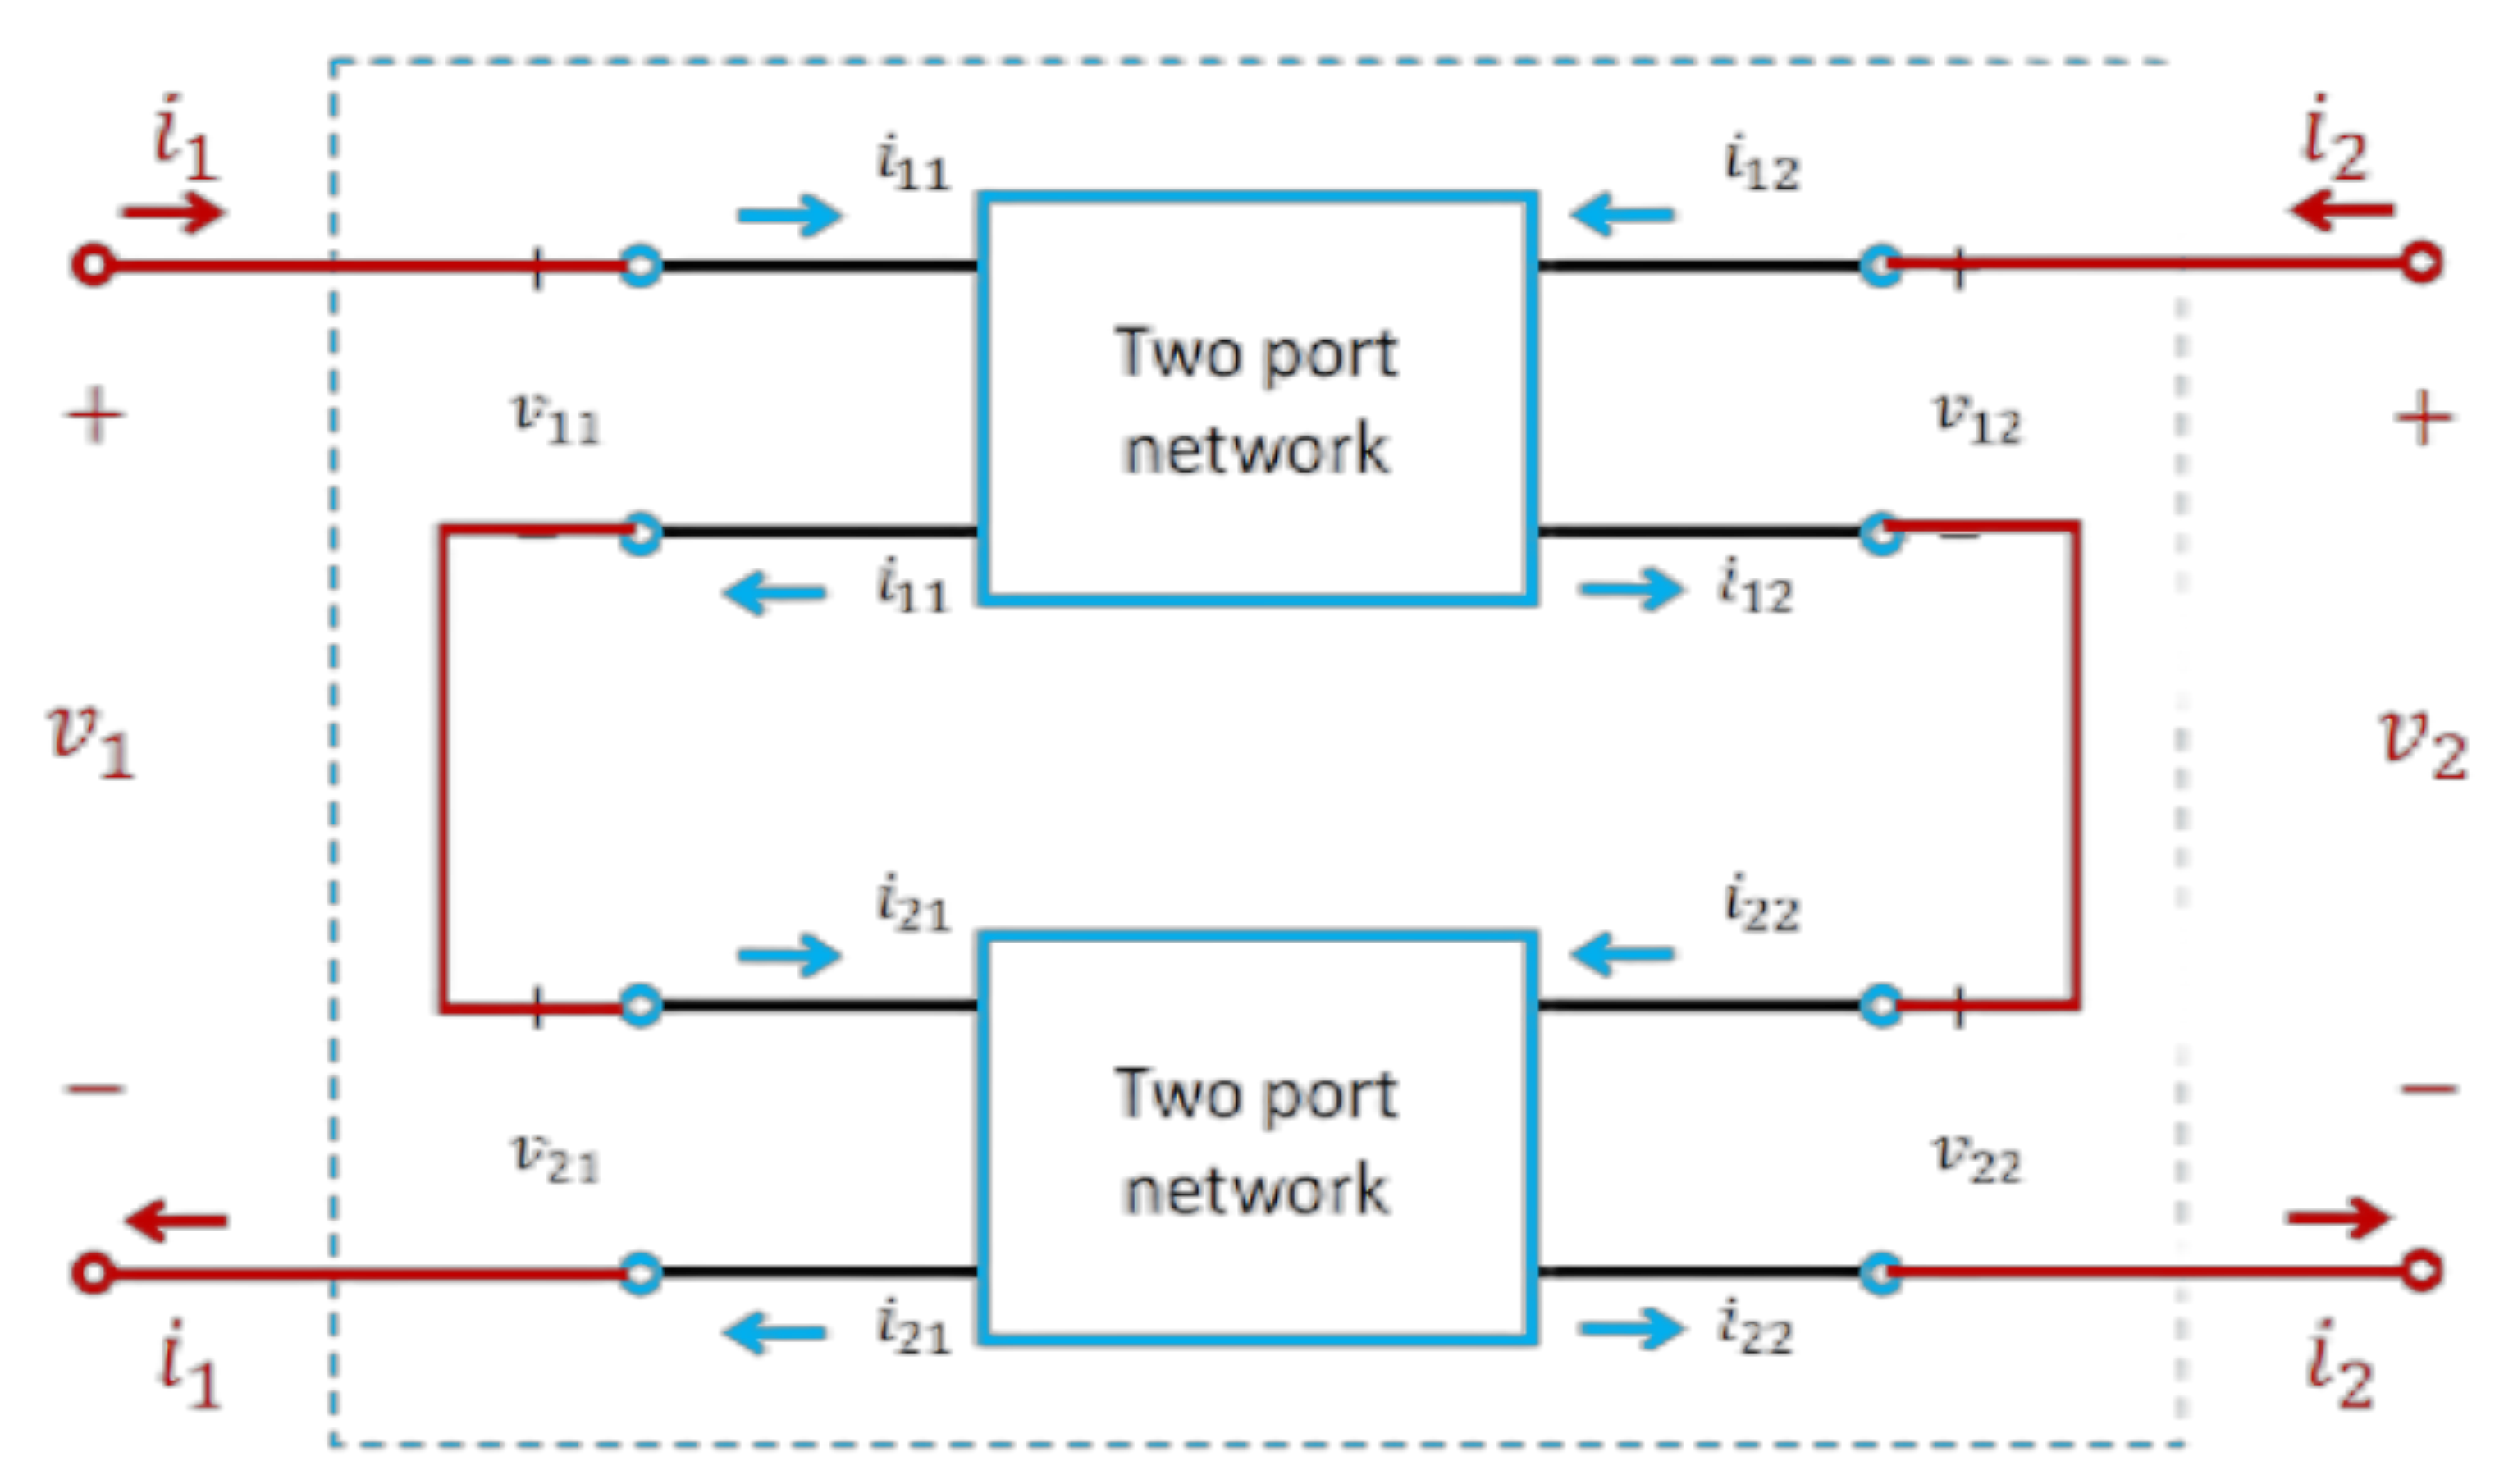
\includegraphics[width=10cm]{双端口网络的串联.png}
	\caption{双端口网络的串联}\label{Pic: 双端口网络的串联}
	\vspace{-1.5em}
	\end{center}
\end{figure}

类似,双端口网络的并联如图~\ref{Pic: 双端口网络的并联}~所示,其伏安特性有
\begin{equation*}
	\begin{bmatrix}
		i_1 \\ i_2
	\end{bmatrix}=\begin{bmatrix}
		i_{11} \\ i_{12}
	\end{bmatrix}+\begin{bmatrix}
		i_{21} \\ i_{22}
	\end{bmatrix}=\symbf{Y}_1\begin{bmatrix}
		v_{11} \\ v_{12}
	\end{bmatrix}+\symbf{Y}_2\begin{bmatrix}
		v_{21} \\ v_{22}
	\end{bmatrix}=(\symbf{Y}_1+\symbf{Y}_2)\begin{bmatrix}
		v_1 \\ v_2
	\end{bmatrix}
\end{equation*}
即其$Y$参数
\begin{equation*}
	\symbf{Y}_\text{并}=\symbf{Y}_1+\symbf{Y}_2
\end{equation*}

\begin{figure}[ht!]
	\begin{center}
	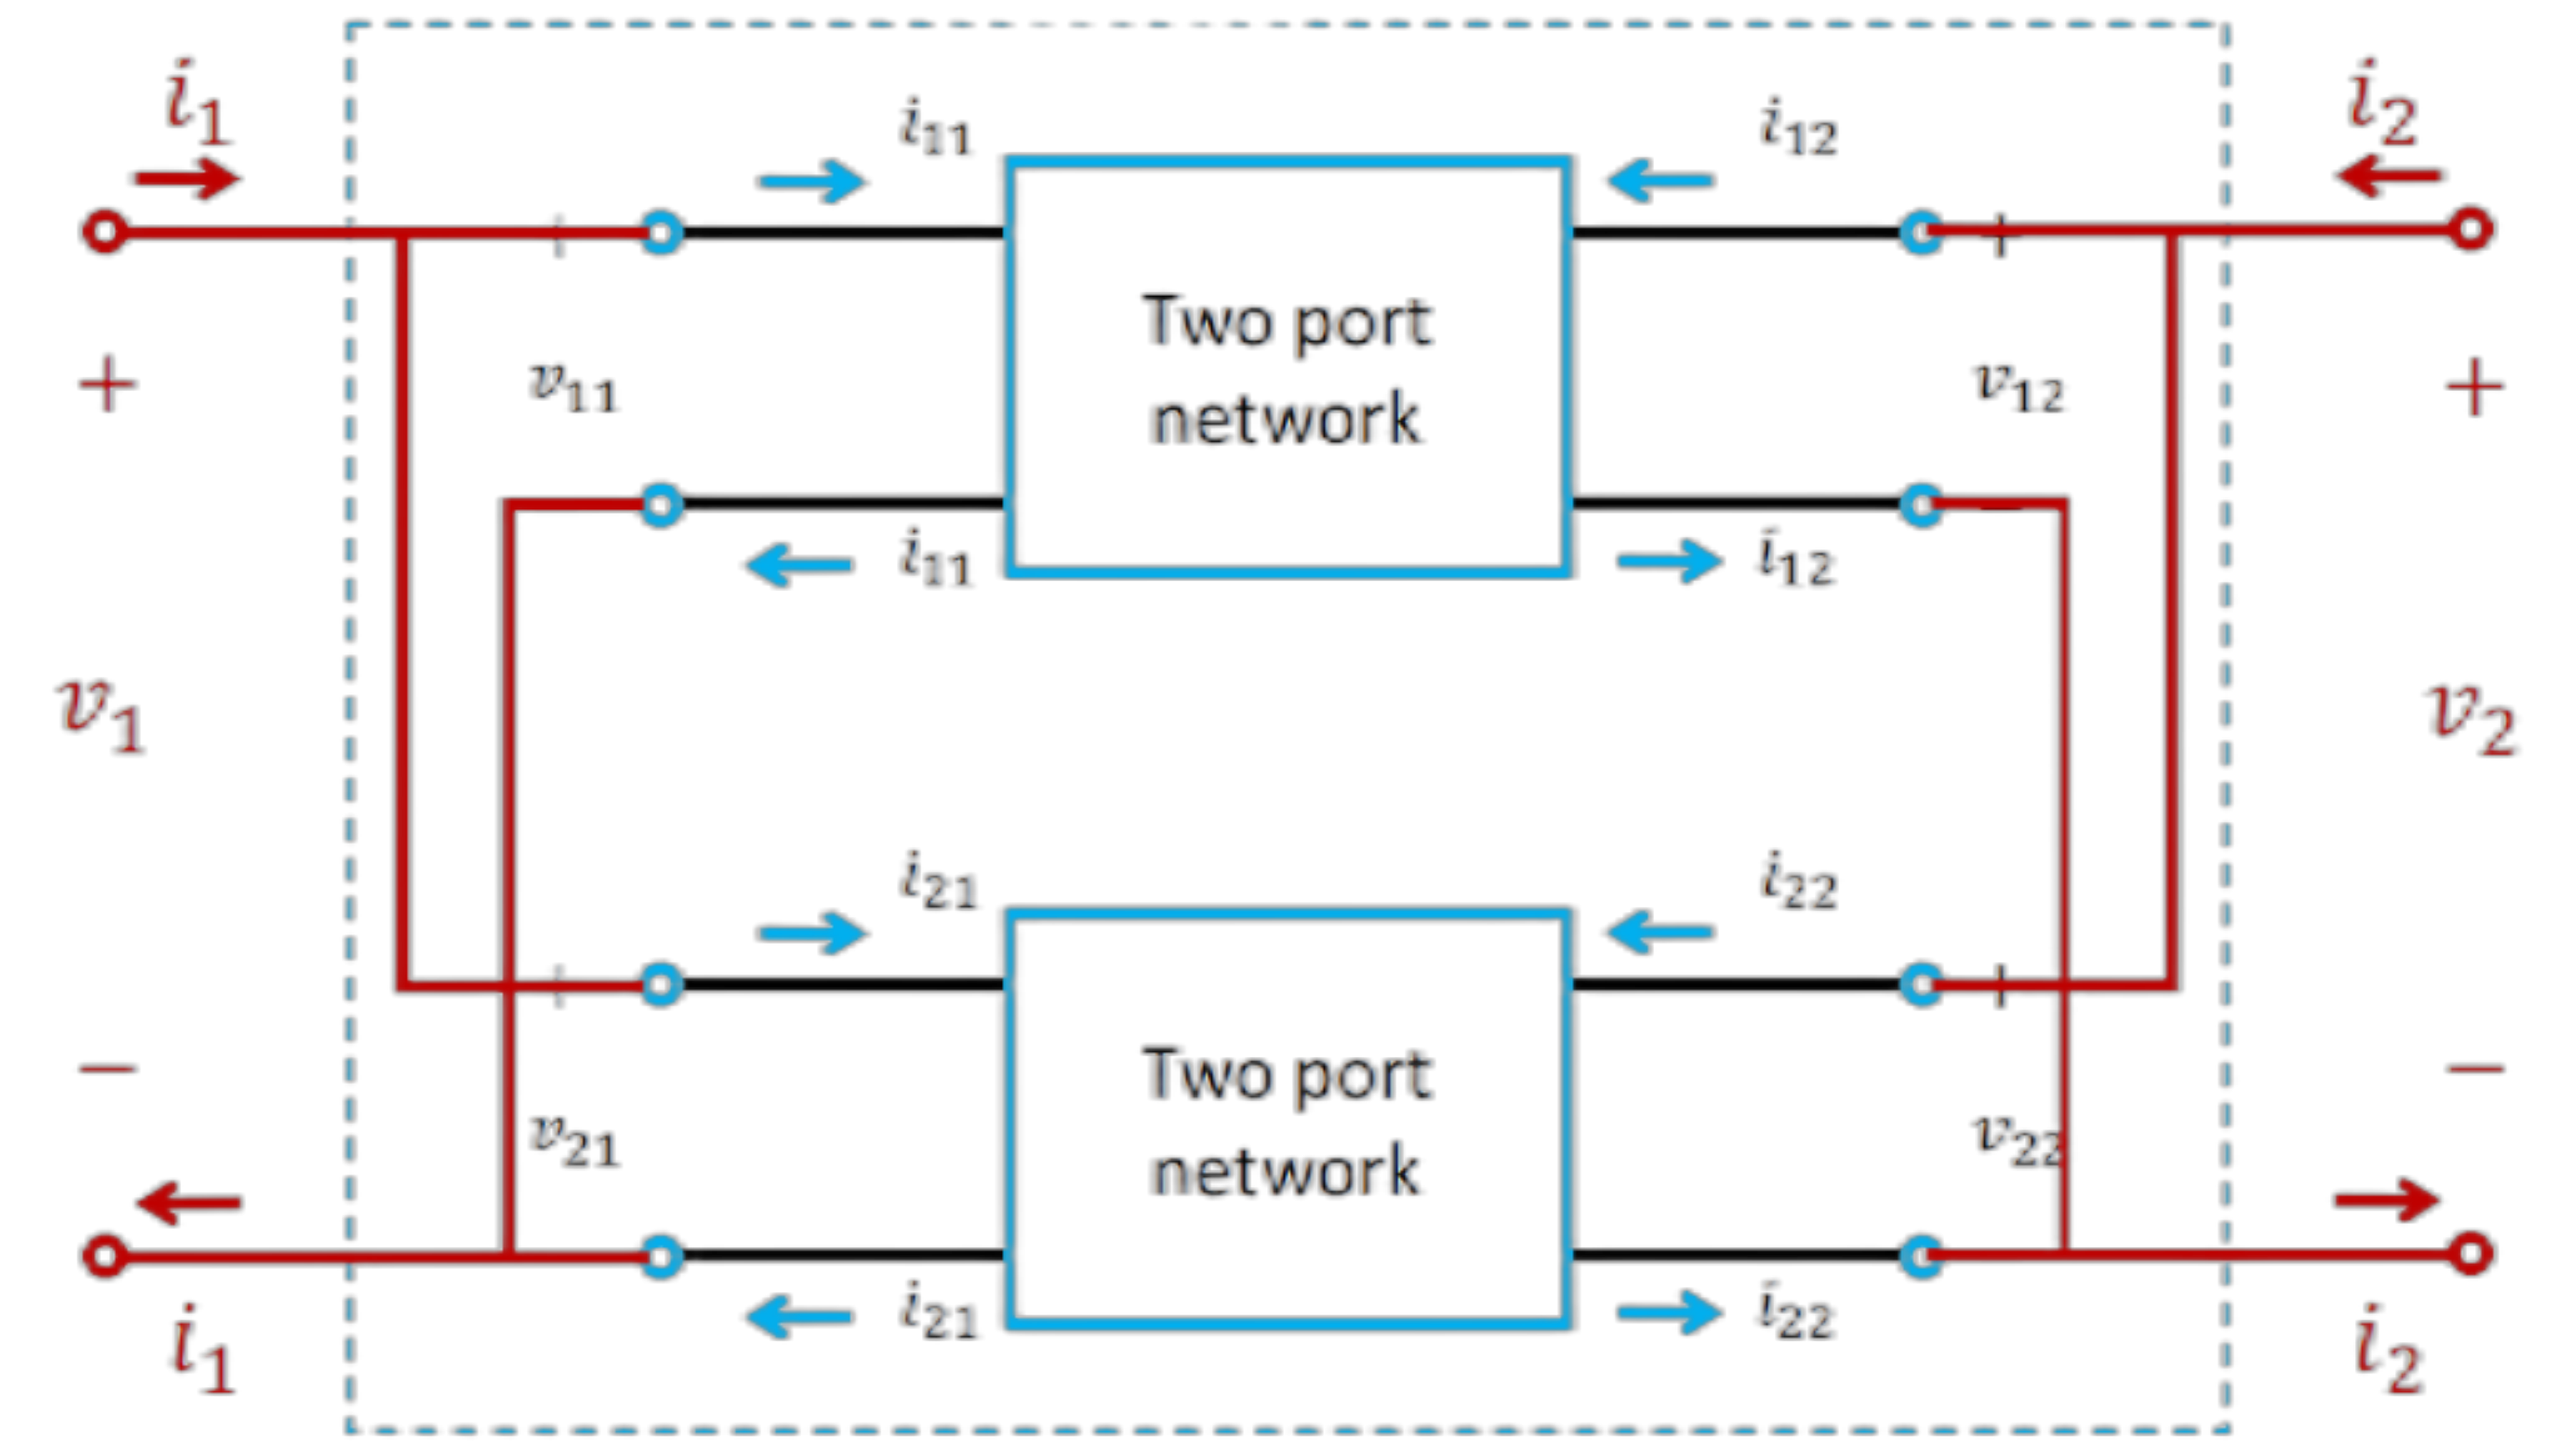
\includegraphics[width=10cm]{双端口网络的并联.png}
	\caption{双端口网络的并联}\label{Pic: 双端口网络的并联}
	\vspace{-1.5em}
	\end{center}
\end{figure}

















%----------------------------------------------------------
\newpage
\appendix
\section{常见词汇中英文对照表}
\begin{longtable}{p{170pt}<{\centering}p{170pt}<{\centering}}
		\toprule
		\textbf{English} & \textbf{中文}\\
		\midrule
	\endfirsthead
		&\hfill{\small\kai 续表}\\
		\toprule
		\textbf{English} & \textbf{中文}\\
		\midrule
	\endhead
		\bottomrule
	\endfoot
	Active Devices&有源器件\\
	Amplification&放大\\
	Angular frequency&角频率\\
	Base Region&基区\\
	Bistable Circuit&双稳态电路\\
	Bode plot&波特图\\
	Body effect&体效应\\
	Branch&支路\\
	Capacitor&电容器\\
	Channel&通道\\
	Charge&电荷\\
	Circuit Equation&电路方程\\
	CMOS Inverters&CMOS 反相器\\
	Collector Region&集电区\\
	Complementary MOS (CMOS)&互补金属-氧化物-半导体\\
	Complementary Solution&补充解\\
	Complex Power&复功率\\
	Conductance&电导率\\
	Conductivity&导电性\\
	Covalent bonds&共价键\\
	Crossover network&分频网络\\
	Crystal Oscillator&晶体振荡器\\
	Current&电流\\
	Current density&电流密度\\
	Cutoff&截止\\
	Damping Factor&阻尼因子\\
	Decibel&分贝\\
	Depletion Region&耗尽区\\
	Differential Equation&微分方程\\
	Diffusion current&扩散电流\\
	Digital Switches&数字开关\\
	Doped semiconductors&掺杂半导体\\
	Drift current&漂移电流\\
	Dynamic Logic Circuits&动态逻辑电路\\
	Dynamic RAM (DRAM) Cell&动态随机存取存储器单元\\
	Electric Devices&电子器件\\
	Electric field&电场\\
	Electron mobility&电子迁移率\\
	Emitter Region&发射区\\
	Energy&能量\\
	Enhancement-type&增强型\\
	Equivalent circuits&等效电路\\
	Extraordinary Node&非普通节点\\
	Feedback Loop&反馈回路\\
	Field-Effect Transistor (FET)&场效应晶体管\\
	Forward Bias&正向偏置\\
	Free electron&自由电子\\
	Frequency-domain&频域\\
	Gate&栅极\\
	Ground&接地\\
	High pass filter&高通滤波器\\
	Hole mobility&空穴迁移率\\
	Homogeneity&同质性\\
	Impedance&阻抗\\
	Independent sources&独立源\\
	Inductor&电感器\\
	Input Bias Current&输入偏置电流\\
	Input Impedance&输入阻抗\\
	Input Offset Current&输入偏移电流\\
	Integrated Circuit (IC)&集成电路\\
	Integrator&积分器\\
	Kirchhoff's Law&基尔霍夫定律\\
	KVL/KCL&基尔霍夫电压/电流定律\\
	Linear circuit&线性电路\\
	Linear Devices&线性器件\\
	Logic-Gate Circuits&逻辑门电路\\
	Low pass filter&低通滤波器\\
	Lumped Matter Discipline (LMD)&集总物质规律\\
	Magnetic field&磁场\\
	Magnetic Flux&磁通量\\
	Memory Circuits&存储电路\\
	Mesh-current method&回路电流法\\
	Metal-Oxide-Semiconductor (MOS)&金属-氧化物-半导体\\
	Negative Feedback&负反馈\\
	Negative Resistance&负阻抗\\
	NMOS transistor&NMOS 晶体管\\
	Node&节点\\
	Node-voltage method&节点电压法\\
	Noise Margin&噪声裕度\\
	Non-linear Devices&非线性器件\\
	Norton's theorem&诺顿定理\\
	Ohm's Law&欧姆定律\\
	Operational Amplifier&运算放大器\\
	Oscillation&振荡\\
	Overdamped&过阻尼\\
	Parasitic capacitance&寄生电容\\
	Passive Devices&无源器件\\
	Permittivity&介电常数\\
	Phase&相位\\
	PMOS transistor&PMOS 晶体管\\
	Positive Feedback&正反馈\\
	Power&功率\\
	Power Consumption&功耗\\
	Propagation Delay&传播延迟\\
	Quality factor&品质因数\\
	Ramp Function&斜坡函数\\
	Reactive Power&无功功率\\
	Resistance&电阻\\
	Resistor&电阻器\\
	Resonate Frequency&共振频率\\
	Reverse Bias&反向偏置\\
	Saturation Mode&饱和模式\\
	Saturation Region&饱和区域\\
	Schmitt Trigger&施密特触发器\\
	Semiconductors&半导体\\
	Signal Generators&信号发生器\\
	Silicon crystal&硅晶体\\
	Sinusoidal Function&正弦函数\\
	Source&源极\\
	Static RAM (SRAM) Cell&静态随机存取存储器单元\\
	Steady State&稳态\\
	Step Function&阶跃函数\\
	Substrate (Body)&衬底\\
	Superposition&叠加\\
	Thévenin's theorem&戴维南定理\\
	Threshold voltage&阈值电压\\
	Time Constant&时间常数\\
	Transconductance&跨导\\
	Transfer function&传递函数\\
	Transient Circuit Analysis&瞬态电路分析\\
	Tunnel Diode&隧道二极管\\
	Underdamped&欠阻尼\\
	Voltage&电压\\
	Voltage division&电压分压\\
	Voltage Source&电压源\\
\end{longtable}

\newpage
\section{Cadence Virtuoso电路仿真基本用法}

\subsection{启动}

\subsubsection{连接MobaXterm服务器}

\verb|mkdir|:创建文件夹。

\verb|cd|:打开文件夹。

\verb|virtuoso &|:打开Virtuoso。

\subsubsection{新建Virtuoso库}

\textsf{Tools}$\rightarrow$\textsf{Library Manager}打开Virtuoso库管理器对话框「Library manager」,然后\textsf{File}$\rightarrow$\textsf{New}$\rightarrow$\textsf{Library}打开新建库对话框「New Library」。

在New Library界面为library命名,勾选Reference existing technology library,将库\textsf{Analoglib}移入Reference Technology Libraries。

\subsubsection{新建Cell图}

在Library manager界面选中刚才新建的library,单击\textsf{File}$\rightarrow$\textsf{New}$\rightarrow$\textsf{Cell View},在弹出的「New File」窗口中\textsf{Cell}项为Cell命名,同时确认\textsf{Library}选项是刚才新建的library、\textsf{type}选项是\textsf{schematic}。点击\textsf{OK}。此时自动进入到原理图界面。

\subsection{绘图}

\subsubsection{开关}

开关\textsf{switch}实际上是一个电磁继电器,开关的开合由线圈中是否有从$+$到$-$的电流决定。










%----------------------------------------------------------
\end{document}




